\documentclass[dissertation.tex]{subfiles} 
\begin{document}

\chapter{The Compact Muon Solenoid Experiment}
\label{chap:The Compact Muon Solenoid Experiment}

%keep repeating references to the detector paper?
\textcolor{red}{\textbf{Keep repeating references to the detector paper?}}

The Compact Muon Solenoid (CMS) detector sits at point 5 of the LHC ring, diametrically opposite the ATLAS detector at point 1.  It is a 4$\pi$ hermetic general purpose detector, meaning that it has the capability to detect charged and neutral hadrons, photons, electrons, muons, taus, neutrinos, and non-Standard-Model particles predicted to escape the detector with good efficiency over a large range of rapidity.  Its main distinguishing feature is a superconducting solenoid that provides a 3.8T magnetic field parallel to the beam line.  This strong magnetic field allows precise determination of the momentum and charge of muons and electrons up to a momentum of $\sim$1 TeV.

The origin of the CMS coordinate system is at the nominal interaction point.  The $y$-axis points skyward, the $x$-axis points towards the center of the LHC ring, and the $z$-axis points counterclockwise along the LHC ring.  $r$ denotes radial distances from the beam line, $\phi$ is the azimuthal angle measured with respect to the positive $x$-axis, and $\theta$ is the polar angle measured with respect to the positive $z$-axis.  The \textit{pseudorapidity} $\eta$ is defined as $\eta = -\ln\tan(\theta/2)$, and is a good approximation to rapidity $y = (1/2)\ln((E + p_{z}c)/(E - p_{z}c))$ for relativistic particles.  The transverse momentum and energy ($p_{T}$ and $E_{T}$) of a particle are defined as $p_{T} = p\cos\phi$ and $E_{T} = E\cos\phi$, where $p$ and $E$ are the magnitude of the particle's momentum vector and the particle's total energy, respectively.  A depiction of the CMS coordinate system is shown in Figure~\ref{fig:CMS_coordinate_system}.

\begin{figure}
	\centering
	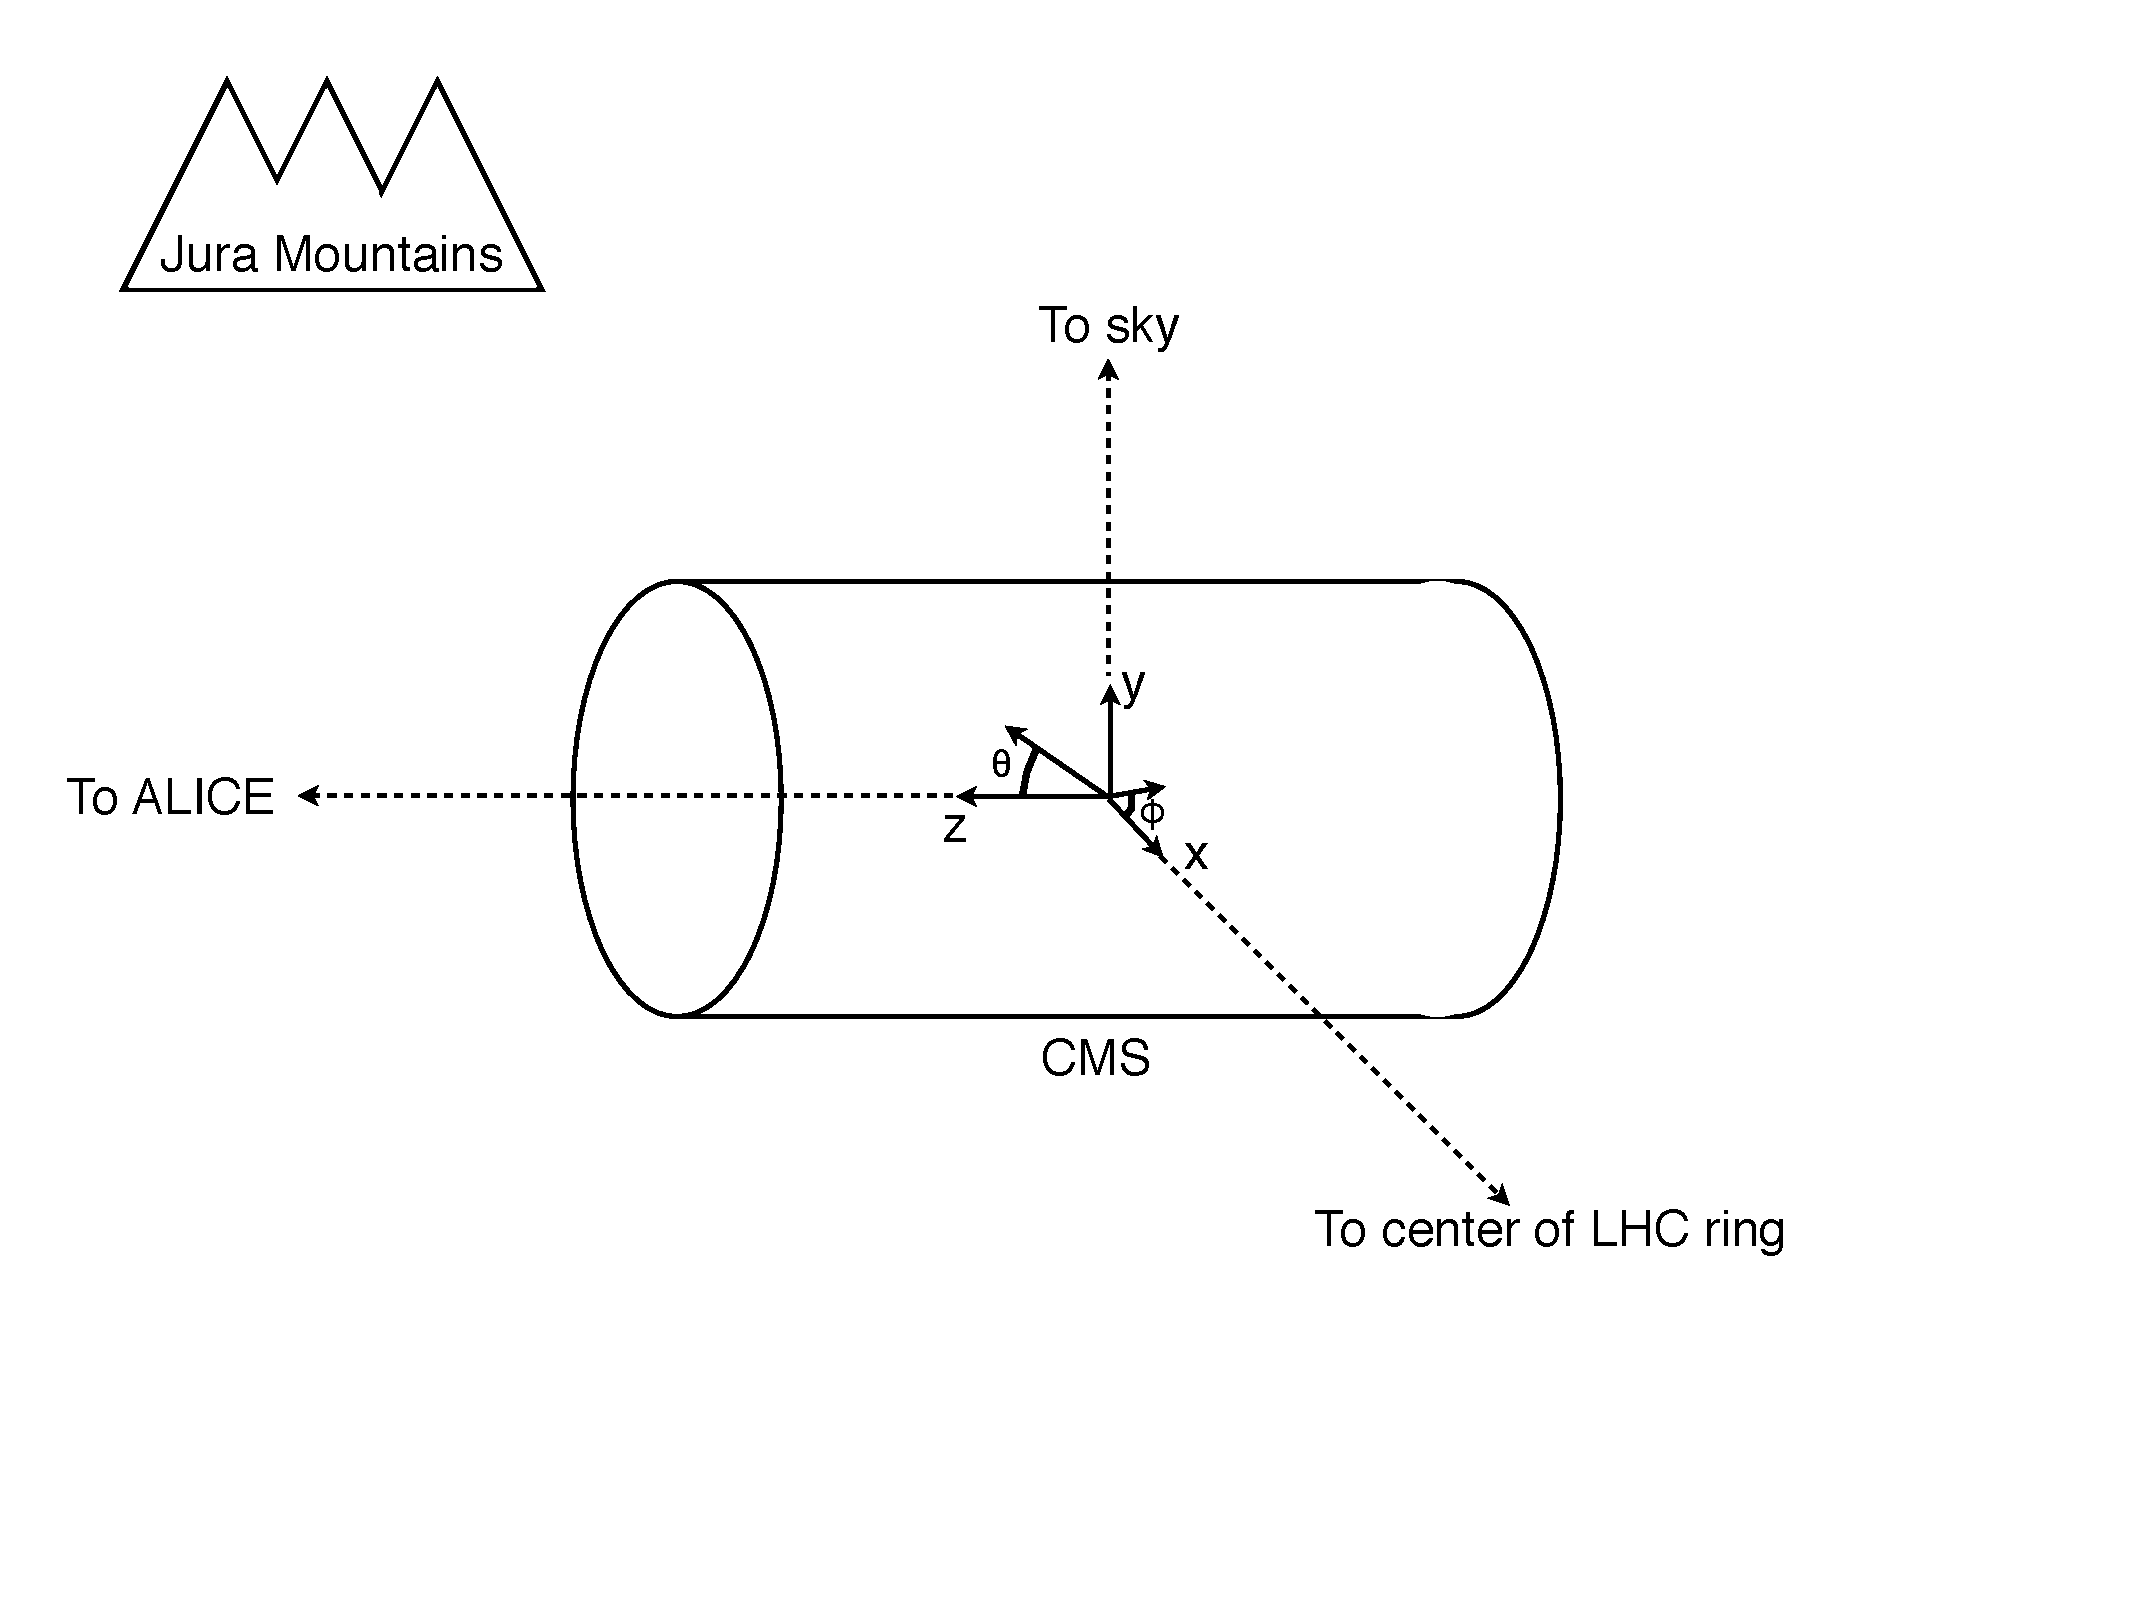
\includegraphics[scale=0.5]{CMS_coordinate_system}
	\caption{CMS coordinate system.}
	\label{fig:CMS_coordinate_system}
\end{figure}

The CMS sub-detectors are arranged in concentric cylindrical layers, plus ``endcaps," around the beam line, as shown in Figure~\ref{fig:CMS_cutaway}.  Closest to the beam line are three layers of silicon pixel detectors, with the innermost at radius 4.4 cm and outermost at radius 10.2 cm \cite{CMS_detector_paper}.  Including the pixel endcaps, the total pixel coverage extends to $\eta$ = 2.5 \cite{CMS_detector_paper}.  The pixel detector plays in important role in determining the proton-proton interaction position (\textit{beam spot}) and the impact parameters of charged particle trajectories, and is critical for the measurement of decay positions some distance from the beam spot (\textit{displaced vertices}), such as those due to the showering and hadronization of a $b$ quark.

\begin{figure}
	\centering
	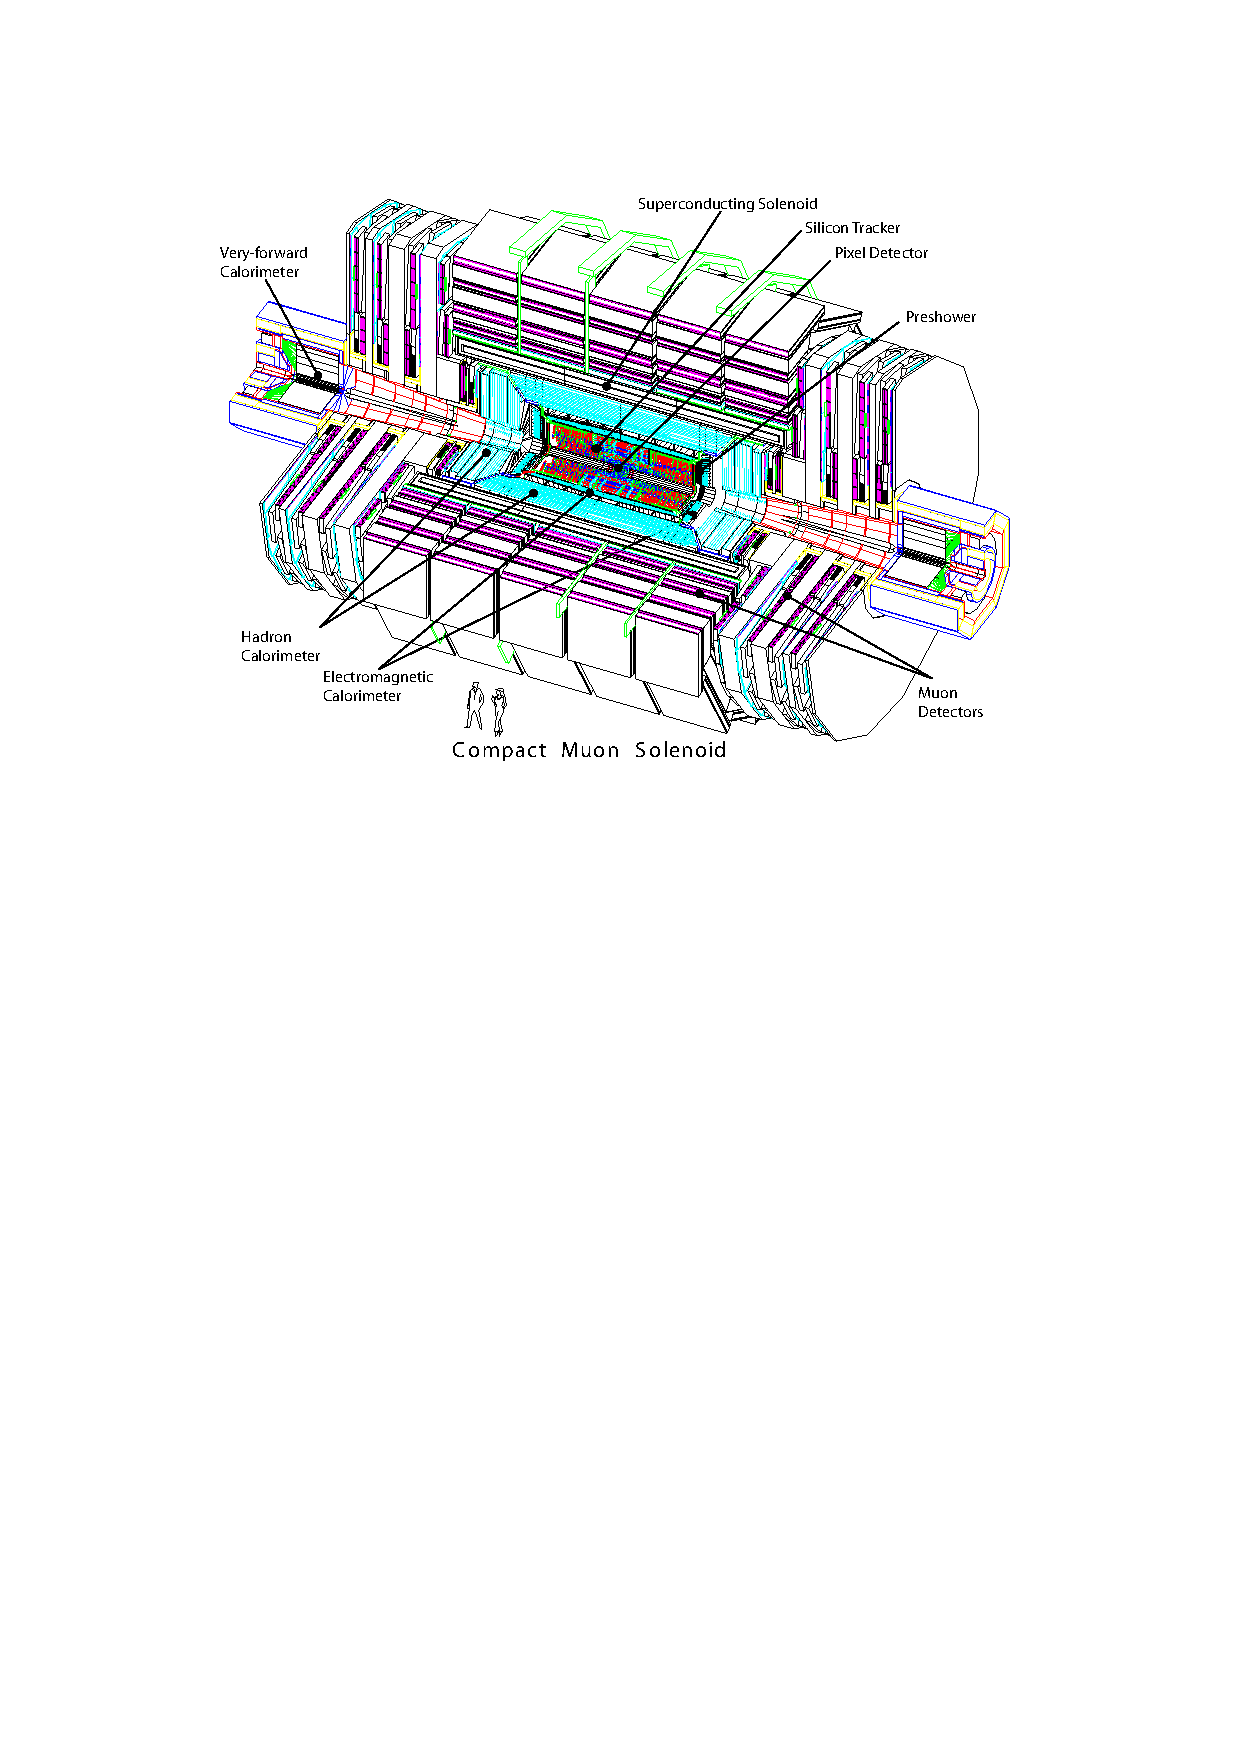
\includegraphics[scale=1.0]{CMS_cutaway}
	\caption{Cutaway view of CMS.  Reprinted from Fig. 1.1 of ref. \cite{CMS_detector_paper}.}
	\label{fig:CMS_cutaway}
\end{figure}

The 10 next layers of CMS are comprised of silicon microstrip detectors, with the outermost layer at a radius of 1.3 m from the beam line \cite{CMS_detector_paper}.  As for the pixel detectors, the silicon strip endcaps extecnd tracking coverage to $\eta$ = 2.5.  The silicon microstrip layers are the workhorse of the CMS tracking system, and provide excellent charged particle momentum resolution and track finding efficiency.

Outside the tracking detectors are the calorimeters, starting with the single-layer lead tungstate crystal electromagnetic calorimeter at a radius of 1.3 m from the beam line (location of crystal front faces) \cite{CMS_detector_paper}.  Each crystal is 23 cm long, corresponding to 25.8 radiation lengths ($\mbox{X}_{0}$).  The crystal dimensions are such that most of one electromagnetic shower, and no more, can be contained in a single crystal, leading to excellent energy resolution for photons and electrons.  The electromagnetic calorimeter radial and endcap layers cover a pseudorapidity range up to 3.0.  A lead/silicon sampling calorimeter sits in front of the crystal endcaps to provide better rejection of neutral pions.

The last layer of calorimetry inside the solenoid is the brass/scintillator sampling hadronic calorimeter, which has a radial extent from 1.77-2.95 m \cite{CMS_detector_paper}.  The hadronic barrel and endcap calorimeters cover up to $|\eta|$ = 3.0, while the iron/quartz-fiber forward hadronic calorimeter covers the region $3.0 \leq |\eta| \leq 5.2$. \footnote{The Centauro and Strange Object Research (CASTOR) and Zero Degree Calorimeter (ZDC) detectors provide additional calorimetry beyond $|\eta| = 5.2$.  However, they are mainly used in the heavy ion and diffractive physics programs of CMS, and play no role in the detection of heavy SUSY particles.  Therefore, they will not be discussed here.}  There is one more layer of hadronic calorimetry outside the solenoid in $|\eta| < 1.3$ which, together with the layers inside the solenoid, provides approximately 12 hadronic interaction lengths of instrumented absorber.  Because of its large $|\eta|$ coverage and depth, the hadronic calorimeter provides good missing transverse energy resolution and accurate measurements of high energy jets.

The iron return yoke of the solenoidal magnetic field is interleaved with muon detectors from 4.1-7.4 m in $r$ and 6.6-10.6 m in $z$, providing muon detection up to $|\eta| = 2.4$ \cite{CMS_detector_paper}.  In the barrel region of $|\eta| < 1.2$, drift tubes are used to read out the muon tracks, while in the endcaps cathode strip chambers are used.  Due to their speed, resistive plate chambers are used throughout the muon system to provide an independent trigger and timing measurement.  Combining the tracker and muon system hits, the momenta and charge of muons up to $p_{T} = 1$ TeV can be precisely reconstructed.

A longitudinal quarter cross-sectional view of CMS is shown in Figure~\ref{fig:CMS_longitudinal_xsec}.  The remainder of this chapter is devoted to explaining the CMS subdetectors and readout systems.  Section~\ref{sec:The Detectors and Their Operating Principles} describes the subdetector technologies and performance benchmarks, while Section~\ref{sec:Triggering, Data Acquisition, and Data Transfer} details the CMS trigger and data acquisition systems and framework for promptly reconstructing and transferring data worldwide.  For a thorough description of CMS, see ref. \cite{CMS_detector_paper}, from which much of the information in the section was culled.

\begin{figure}
	\centering
	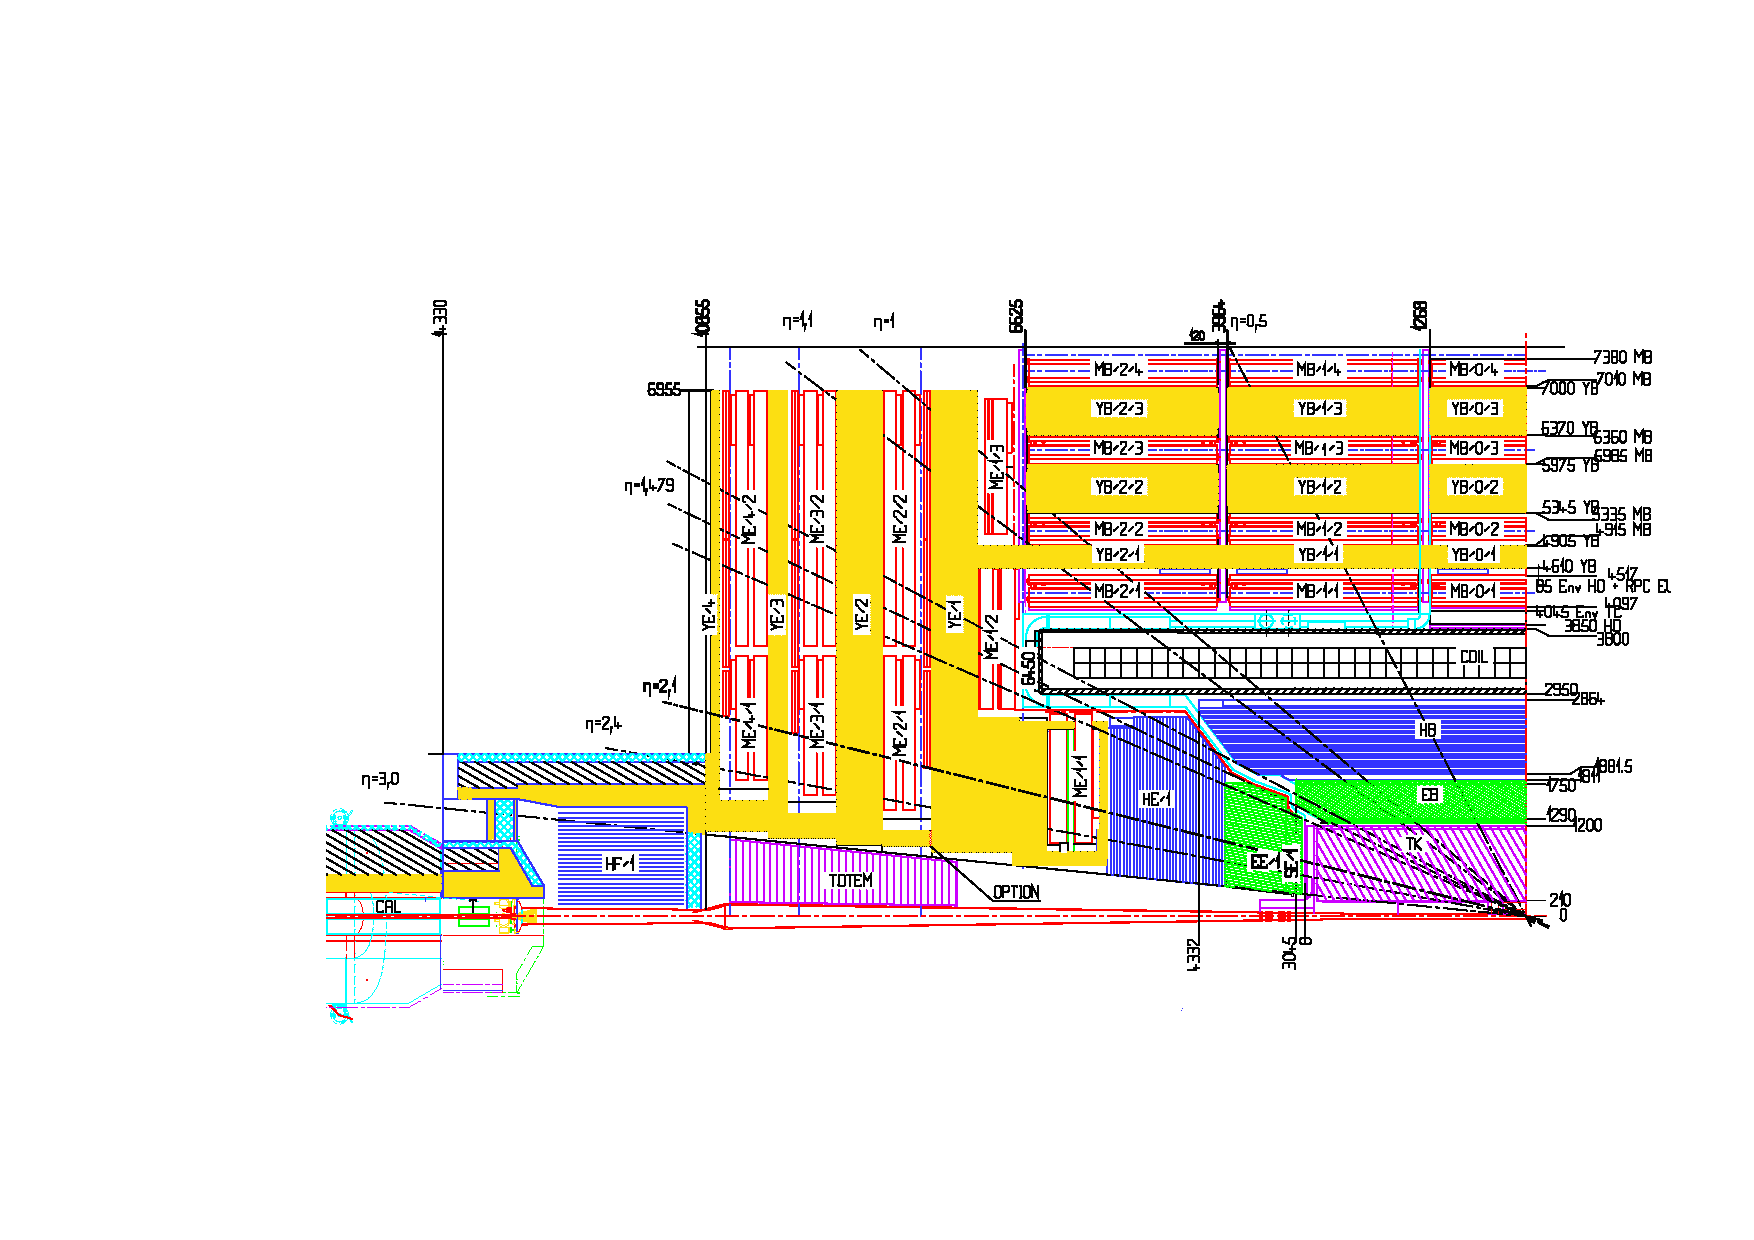
\includegraphics[scale=0.5]{CMS_longitudinal_xsec}
	\caption{Longitudinal quarter cross-sectional view of CMS.  The nominal interaction point is at the lower right-hand corner of the drawing.  The tracker is shown in purple diagonal hashing, the electromagnetic calorimeter in green, the hadronic calorimeter in blue, and the muon stations in red.  The solenoid is shown in black and white and labeled \texttt{COIL}, and the magnet return yoke is shown in yellow.  Radial and longitudinal distances are measured in millimeters.  Reprinted from Fig. CP 1 of ref. \cite{CMS_TDR}.}
	\label{fig:CMS_longitudinal_xsec}
\end{figure}

\section{The Detectors and Their Operating Principles}
\label{sec:The Detectors and Their Operating Principles}

\subsection{Tracking System}
\label{sec:Tracking System}

Given the LHC design instantaneous luminosity, efficient reconstruction of charged particle tracks from transverse momenta of 1 GeV up to 1 TeV can only be achieved with a low occupancy tracker.  For $r < 10$ cm, the hit rate density is highest, leading to the choice of $100\mbox{ }\mu\mbox{m} \times 150\mbox{ }\mu\mbox{m}$ silicon pixel sensors for hit detection.  For $20\mbox{ cm }< r < 110\mbox{ cm}$, the lower hit rate allows the use of silicon strips, with length along $z$ of order centimeters and length along the $r\cdot\phi$ curve of order hundreds of microns.  This design leads to a pixel hit occupancy of $\sim10^{-4}$/pixel/BX and a strip hit occupancy of $\sim10^{-2}$/pixel/BX, where BX refers to 1 LHC bunch crossing \cite{CMS_detector_paper}.

As radiation dose from hadrons accumulates over the lifetime of the tracker, silicon leakage current through the semiconductor junctions increases, heating up the sensors.  Since the leakage current itself depends on temperature, this can lead to \textit{thermal runaway} that damages the detector.  To avoid this, the tracker must be cooled to approximately $-10^{\circ}$C.  Operating at this temperature, the signal:noise ratio in the silicon sensors is 10:1, and should remain at that level over the 10-year lifetime of the tracker \cite{CMS_detector_paper}.

At its thickest ($|\eta|\sim1.5$), the tracker depth (including services) is $\sim1.8X_{0}$, and the depth falls off to $\sim1X_{0}$ in thinner areas.  Unfortunately, the large mass of the tracker degrades somewhat the performance of the electromagnetic calorimeter behind it, as $\sim50$\% of photons will convert to $e^{+}e^{-}$ pairs in the tracker.

\subsubsection{Pixel Detector}
\label{sec:Pixel Detector}

A longitudinal quarter view of the three barrel pixel (BPix) layers and two forward pixel (FPix) disks is shown in Figure~\ref{fig:pixel_longitudinal_quarter_view}.  There are 768 BPix modules in total.  Each BPix layer is divided into 32 $\phi$-wedges, with eight modules per wedge arranged end-to-end in $z$.  The $\phi$-wedges operate nearly independently in terms of clock and readout.  Each FPix disk consists of 24 $\phi$-wedges, with pie-shaped modules attached to the front and back of the disk, for a total of 192 modules.  The front- and back-side modules of the FPix disks are constructed of different sized \textit{plaquettes}, or multi-pixel sensor chips, such that the gaps in the front-side module are covered by plaquette area in the back-side module and vice versa.  An illustration of the BPix and FPix mechanical layouts is given in Figure~\ref{fig:pixel_mechanics}.

\begin{figure}
	\centering
	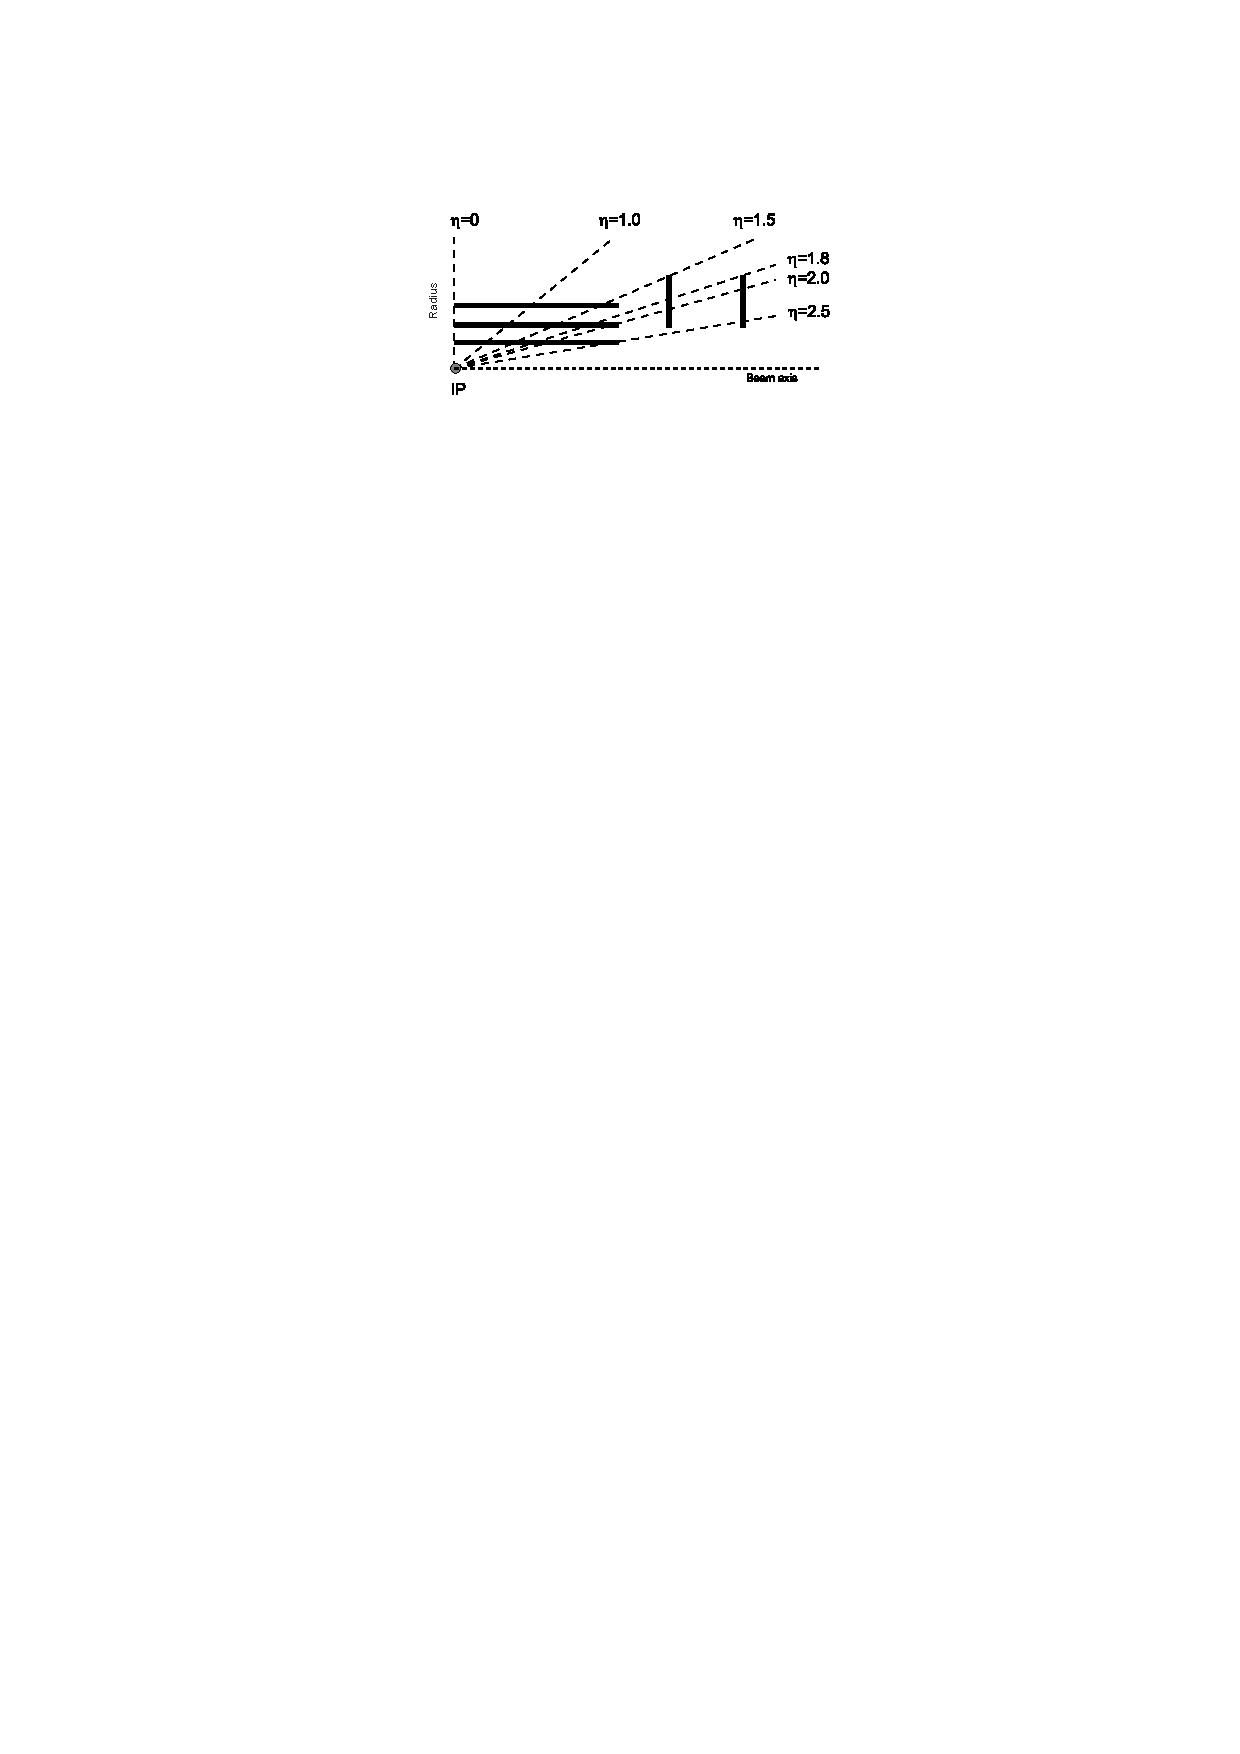
\includegraphics[scale=1.0]{pixel_longitudinal_quarter_view}
	\caption{Longitudinal quarter view of the pixel detector.  Reprinted from Fig. 3.6 of ref. \cite{CMS_detector_paper}.}
	\label{fig:pixel_longitudinal_quarter_view}
\end{figure}

\begin{figure}
	\centering
 	\subfloat[Cutaway view of the barrel pixel layers, showing the three layers and the eight end-to-end modules along $z$.  Reprinted from Fig. 3.11 of ref. \cite{CMS_detector_paper}.]{\label{fig:BPix_mechanics}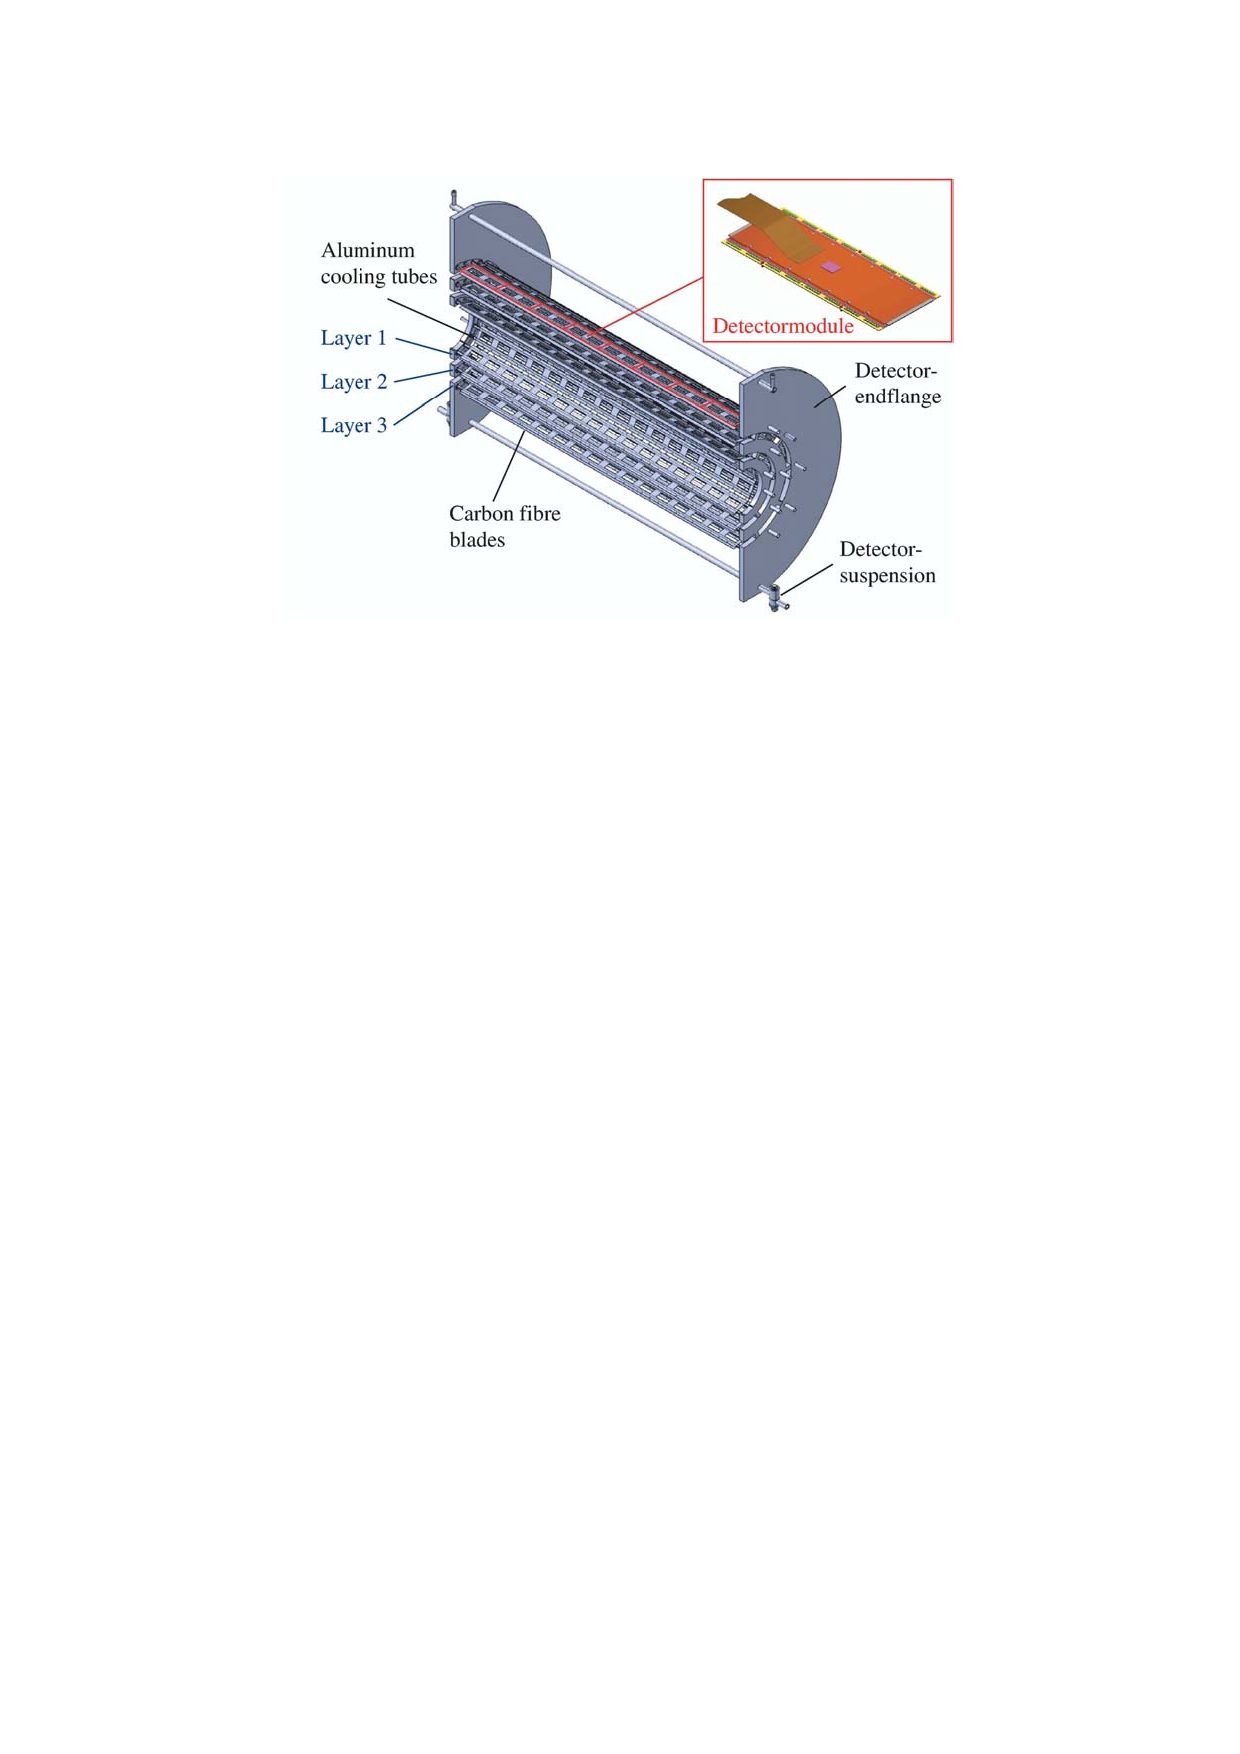
\includegraphics[scale=0.6]{BPix_mechanics}}
	\hspace{1cm}
	\subfloat[Half-disk of the foward pixel detector, showing the 12 pie-shaped module mounts.  Reprinted from Fig. 3.15 of ref. \cite{CMS_detector_paper}.]{\label{fig:FPix_mechanics}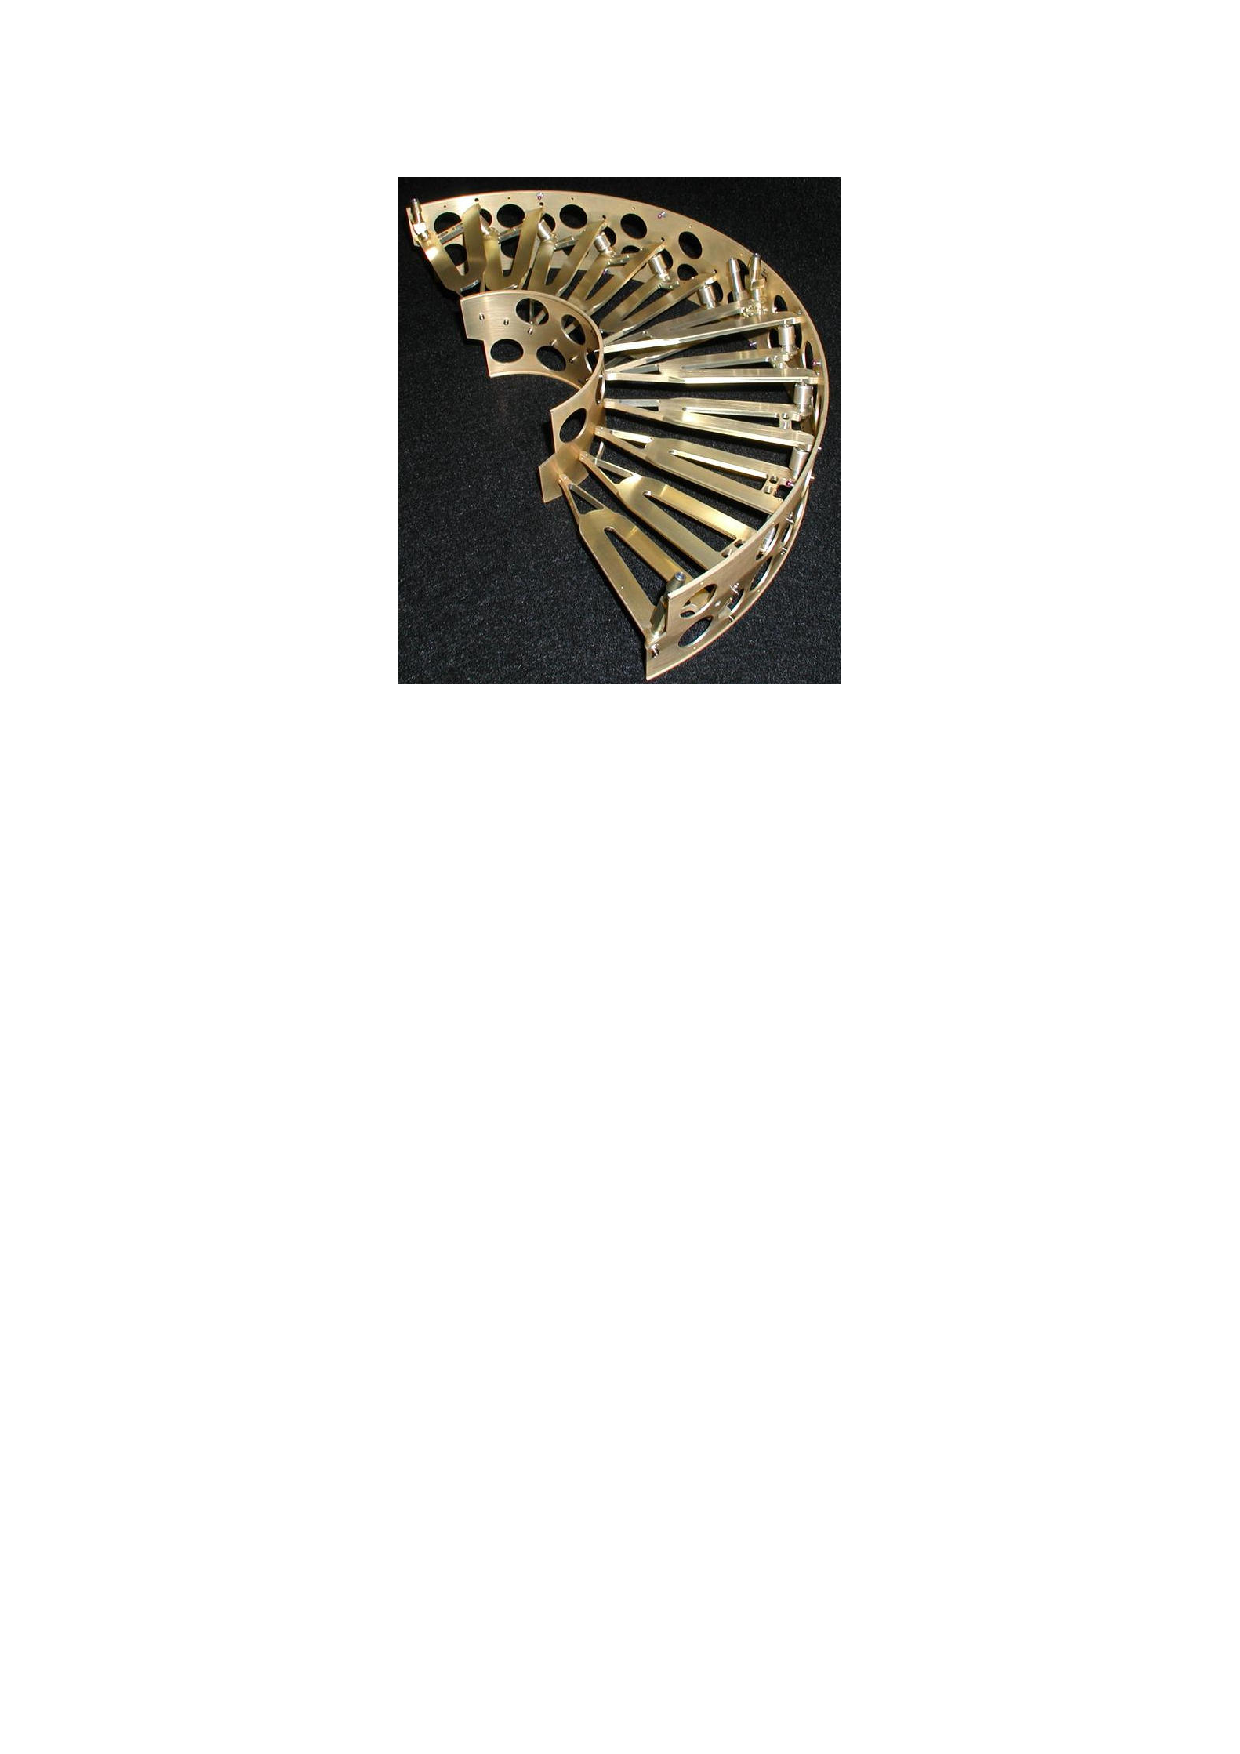
\includegraphics[scale=0.6]{FPix_mechanics}}
	\caption{BPix and FPix mechanical structures.}
	\label{fig:pixel_mechanics}
\end{figure}

%insert reference to BPix Lorentz angle
Since the electric field in the depletion region of the BPix sensors is perpendicular (i.e. pointing along $r$) to the magnetic field of CMS (i.e. pointing along $z$), the charge carriers in the silicon experience a Lorentz drift along $\phi$.  The multi-pixel sensor pitch is such that this causes the charge from one particle hit to be shared among multiple pixels.  Particle hits are reconstructed reading out the analog pixel signal and interpolating between signals in multiple pixels.  This method achieves a 15-20 $\mu\mbox{m}$ spatial resolution, which is comparable to the sensor pitch.  To induce this effect in FPix, the sensor wedges are tilted by the BPix Lorentz angle of $20^{\circ}$ \textcolor{red}{\textbf{(insert reference to BPix Lorentz angle)}} with respect to the $y$-axis.

%bias voltage of the pixels?
%explanantion of electrical isolation of pixels?
Each multi-pixel sensor consists of an array of $52\times80$ n-type pixels implanted onto an n-type substrate with 320 $\mu\mbox{m}$ thickness.  The other face of the substrate is covered with a thin layer of p-type semiconductor.  Except for the outer edges, which are held at ground potential to prevent sparking between the sensor edges and the connected readout chip \cite{pixel_design_paper}, the p-side is reverse biased at \textcolor{red}{\textbf{a few hundred volts}}.  The pixels are held at ground potential.  A particle entering through the p-side will cause a burst of current to flow across the p-n junction.  The charge will be collected by the pixels, which are bump-bonded to the readout.  The BPix and FPix sensors employ slightly different technologies for electrically isolating the individual pixels, but both rely on the idea of surrounding the pixels with a p-type material to provide a p-n junction.  Since both pixel and surrounding p-type material are held at ground potential, the p-n junction acts as a barrier to current flow.  \textcolor{red}{\textbf{Is this right?}}

Each $52\times80$ pixel sensor is bump bonded to a readout chip (ROC).  The ROCs provide zero suppression and amplify,  buffer, and communicate the signals from the sensors.  A single token bit manager (TBM) controls $\sim16$ ROCs in the barrel or $\sim24$ ROCs in the endcaps.  Its purpose is to distribute the clock and trigger to the ROCs (the latter initiates a transmission of the signal further upstream to be assembled into the full event readout of CMS).  The clock and trigger are supplied by the pixel front end controller (pFEC), which interfaces to the central clock and data acquisition systems.  Analog signals that are collected from the pixel front ends are digitized by the pixel front end digitizer (pxFED).  A diagram of the readout system is shown in Figure~\ref{fig:pixel_readout}.

\begin{figure}
	\centering
	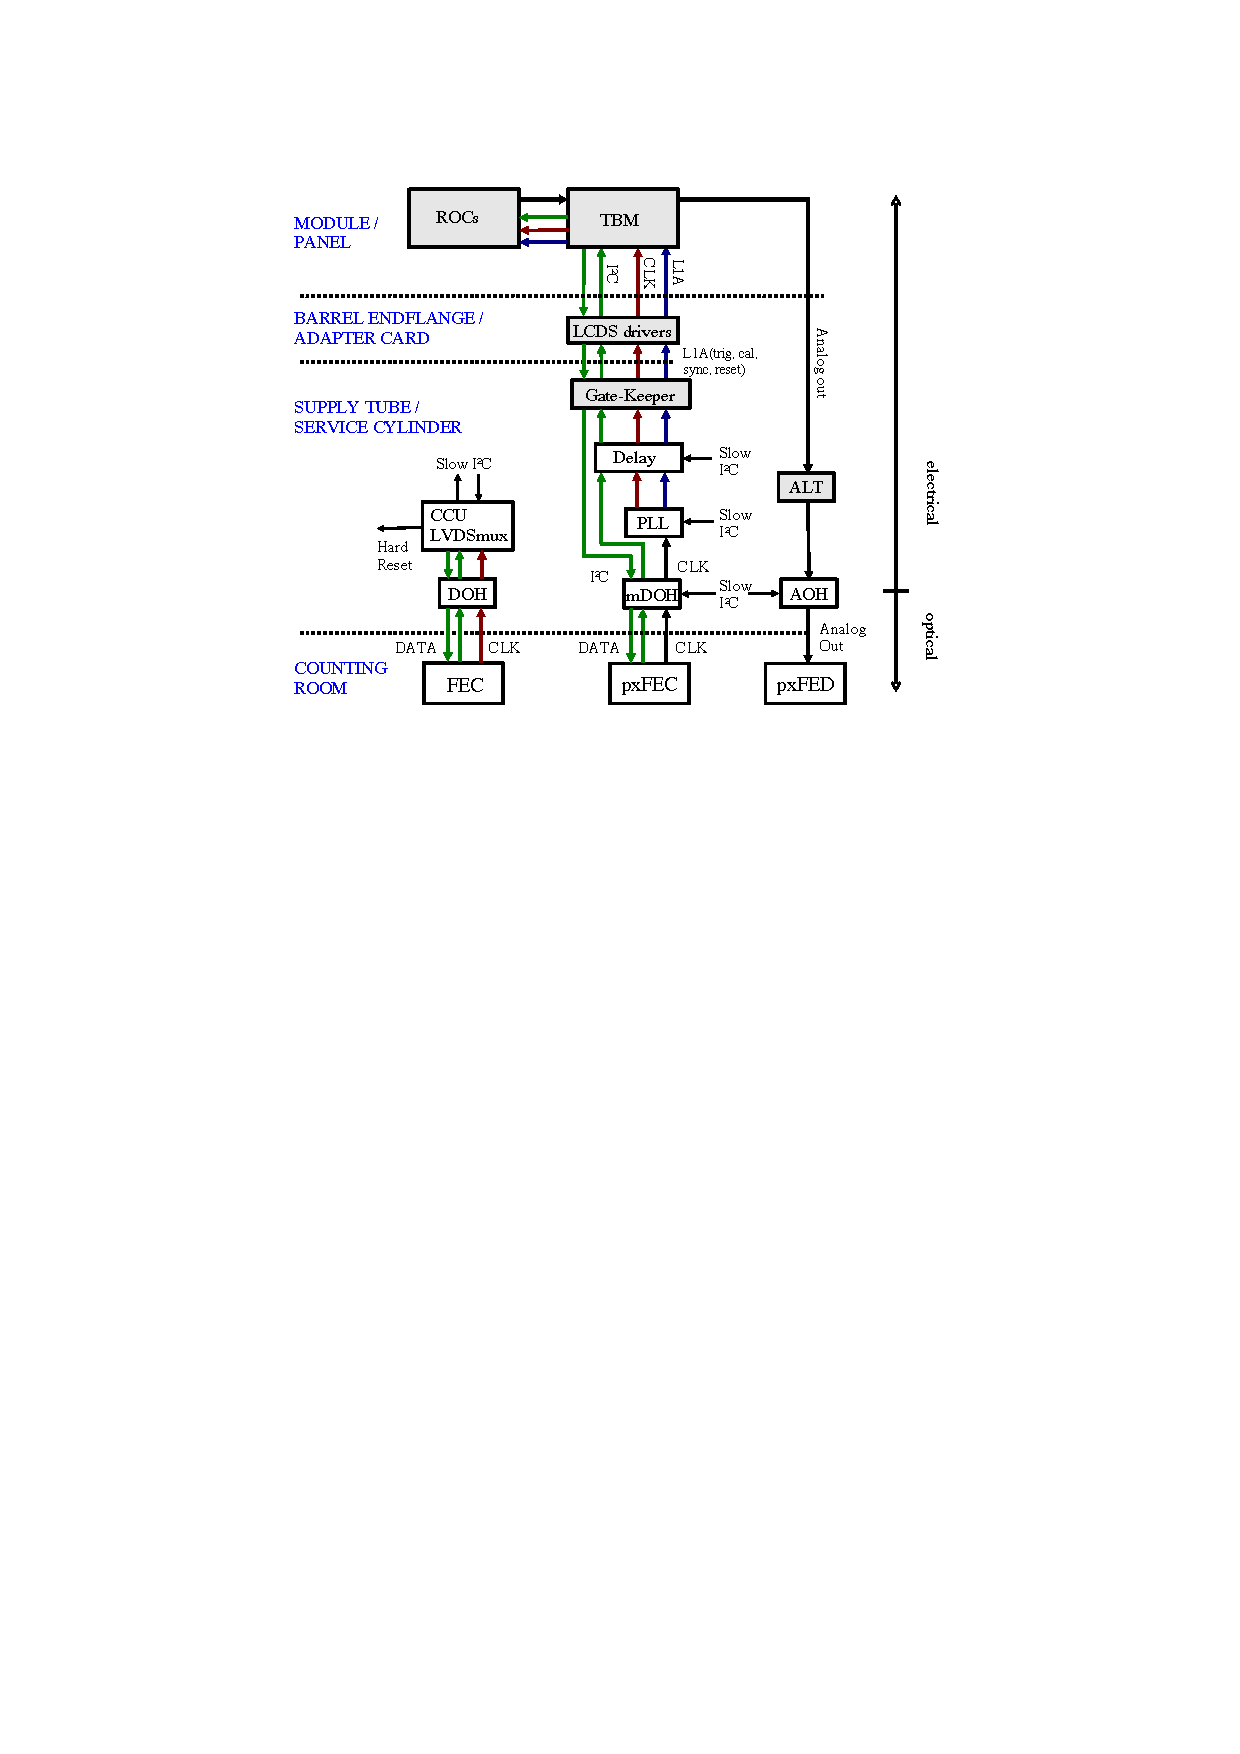
\includegraphics[scale=1.0]{pixel_readout}
	\caption{Pixel control and readout system.  Reprinted from Fig. 3.9 of ref. \cite{CMS_detector_paper}.}
	\label{fig:pixel_readout}
\end{figure}

Figure~\ref{fig:pixel_results} shows some results highlighting the performance of the pixel detector.

\begin{figure}
	\centering
 	\subfloat[BPix hit resolution in the $r\cdot\phi$ coordinate \cite{pixel_DPG_Twiki_rphi_res}.]{\label{fig:pixel_results_rphi_res}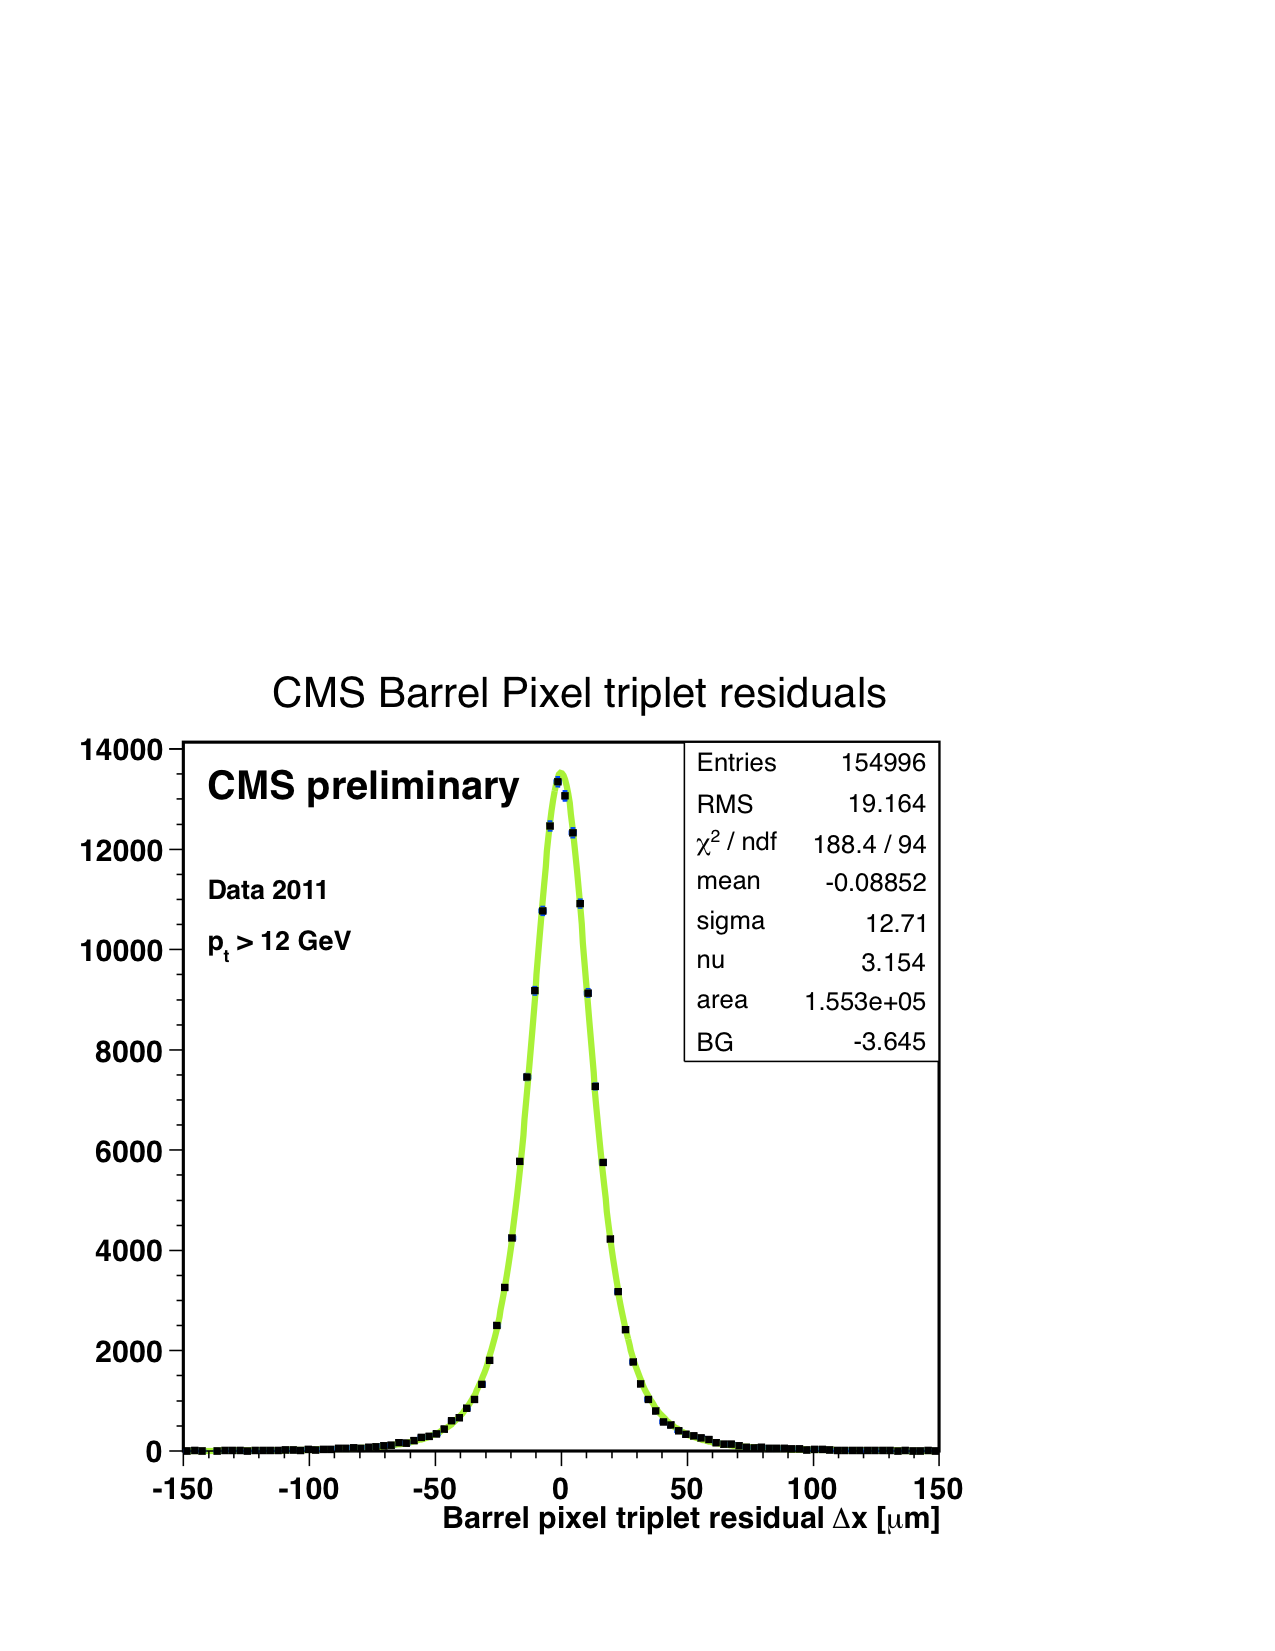
\includegraphics[scale=0.18]{pixel_results_rphi_res}}
	\hspace{1cm}
	\subfloat[BPix hit resolution in the $z$ coordinate vs. track dip angle, showing the effect of charge sharing on resolution \cite{pixel_DPG_Twiki_z_res}.]{\label{fig:pixel_results_z_res}\includegraphics[scale=0.18]{pixel_results_z_res}}
	\hspace{1cm}
	\subfloat[Pixel reconstruction efficiency vs. bias voltage for a group of three wedges in FPix \cite{pixel_DPG_Twiki_eff}.]{\label{fig:pixel_results_eff}\includegraphics[scale=0.18]{pixel_results_eff}}
	\caption{Pixel detector performance highlights.}
	\label{fig:pixel_results}
\end{figure}

\subsubsection{Silicon Strip Tracker}
\label{sec:Silicon Strip Tracker}

The silicon strip tracker is divided into four parts: the inner barrel (TIB) and inner disks (TID), covering the radial extent $20\mbox{ cm} < r < 55\mbox{ cm}$ and $z$ extent $80\mbox{ cm} < |z| < 90\mbox{ cm}$; and the outer barrel (TOB) and endcap (TEC), covering the radial extent $61\mbox{ cm} < r < 108\mbox{ cm}$ and $z$ extent $124\mbox{ cm} < |z| < 282\mbox{ cm}$.  A number of the tracker layers and endcaps hold double-sided strip modules (shown as double lines in Figure~\ref{fig:strip_longitudinal_xsec}), with the rear module tilted at an angle of 100 mrad with respect to the front module, to provide a measurement in two coordinates.  There are a total of 15,148 modules in the tracker, arranged as shown in the longitudinal cross-sectional view of Fig.~\ref{fig:strip_longitudinal_xsec}.  For the TIB and TOB, the modules are arranged in straight rows end-to-end along $z$, with repeating rows covering the full $2\pi$ extent in $\phi$.  In each of the TID disks, the modules are arranged into three concentric circular rings of increasing $r$.  In the TEC, the modules are affixed to $\phi$-wedges called $\textit{petals}$.   One side of the TEC and its petal structure is shown in Figure~\ref{fig:tracker_TEC}.

\begin{figure}
	\centering
	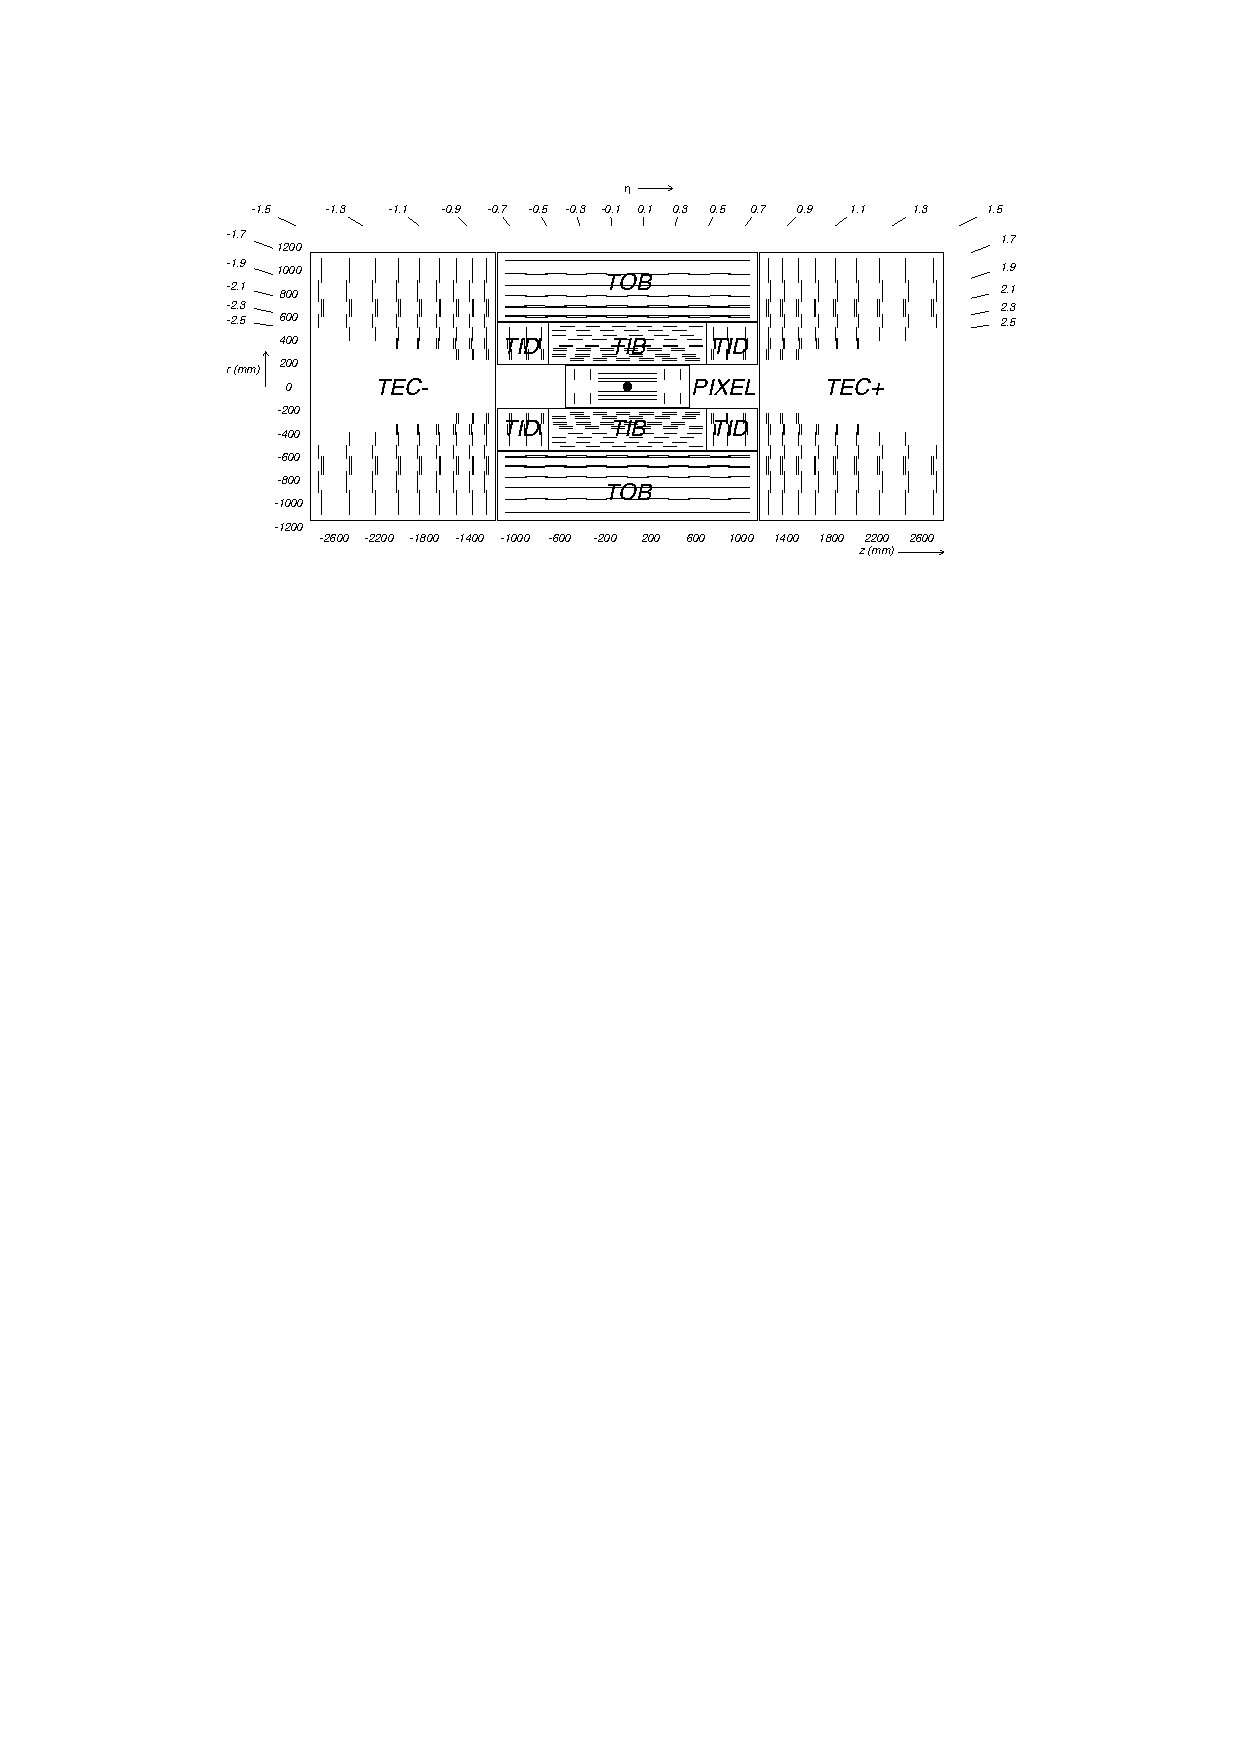
\includegraphics[scale=1.0]{strip_longitudinal_xsec}
	\caption{Longitudinal cross section of the silicon strip detector.  Reprinted from Fig. 3.1 of ref. \cite{CMS_detector_paper}.}
	\label{fig:strip_longitudinal_xsec}
\end{figure}

\begin{figure}
	\centering
	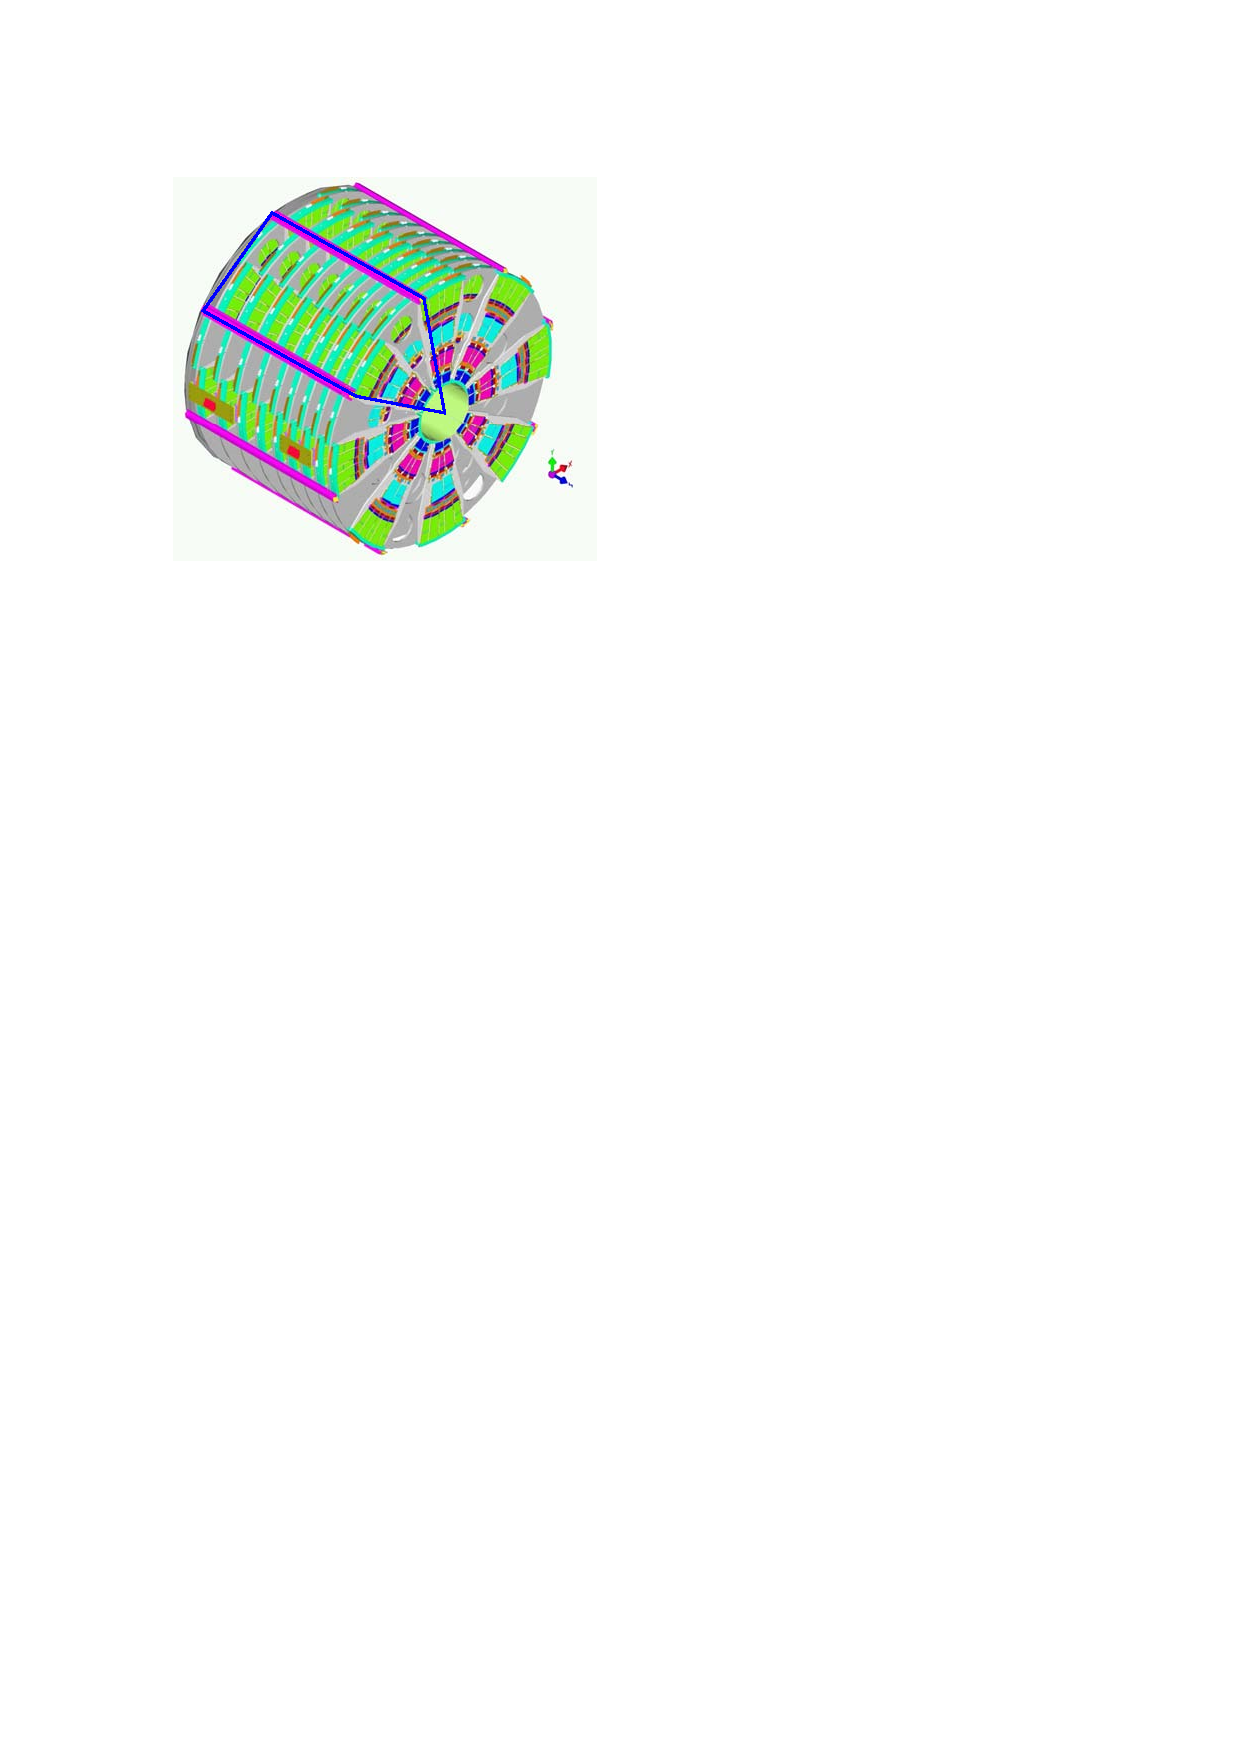
\includegraphics[scale=1.0]{tracker_TEC}
	\caption{View of one tracker endcap, with the outline of a petal shown in blue.  There are nine petals per wedge-shaped sector (one per TEC disk).  Reprinted from Fig. 3.30 of ref. \cite{CMS_detector_paper}.}
	\label{fig:tracker_TEC}
\end{figure}

Like the pixels, the strip sensors generate a signal when current flows across a p-n junction in response to interaction with a charged particle.  Whereas the pixels are n-type implants on an n-type substrate, with a solid p-type rear layer to which the high voltage is connected, the strips are p-type implants on an n-type substrate, with a solid n-type rear layer connecting to the high voltage.  The p-n junction in the strip sensors is at the strip-substrate boundary, whereas in the pixel sensors it is at the boundary between the rear layer and the substrate.  Each sensor has either 512 or 768 electrically isolated strips, with pitch varying from 80-205 $\mu\mbox{m}$ depending on location.  Strip lengths in $z$ range from $\sim10$ to $\sim25$ cm.  Thin (320 $\mu\mbox{m}$) sensors are used in the TIB, TID, and inner four rings of the TEC, while thick (500 $\mu\mbox{m}$) sensors are used in the TOB and the outer rings of the TEC.  The thicker sensors compensate for the increased strip capacitance (and hence electronics noise) of the longer strips in the outer layers/disk of the tracker such that strip signal:noise is maintained above 10 everywhere.

The strips are wire bonded to a front end readout chip called the APV25.  The APV25 amplifies and shapes the strip signals before sending the full analog pulse information to an APVMUX, which multiplexes the output of two APV25s.   Then, the electrical signal from the APVMUX is set differentially a few centimeters to an optical driver, where it is converted to an optical signal and sent to one of the 450 front end drivers (FEDs).  The FEDs convert the signal back to an electrical pulse and digitize it for use in the global event assembly.  As for the pixels, analog readout is used on detector so that hit reconstruction may benefit from charge sharing.

Clock, trigger, and control signals are sent from the front end controllers (FECs) to phase locked loop (PLL) chips on the front ends.  The FECs interface to the global clock and trigger system.  Four or six APV25s, an APVMUX, and a PLL chip all sit on a \textit{hybrid}, two which one thin or two thick sensors are also affixed.  The sensor-hybrid combination and its frame form a module.  Figure ~\ref{fig:tracker_module} shows a diagram of a module, while Figure~\ref{fig:tracker_readout} shows a block diagram of the strip readout architecture.

\begin{figure}
	\centering
	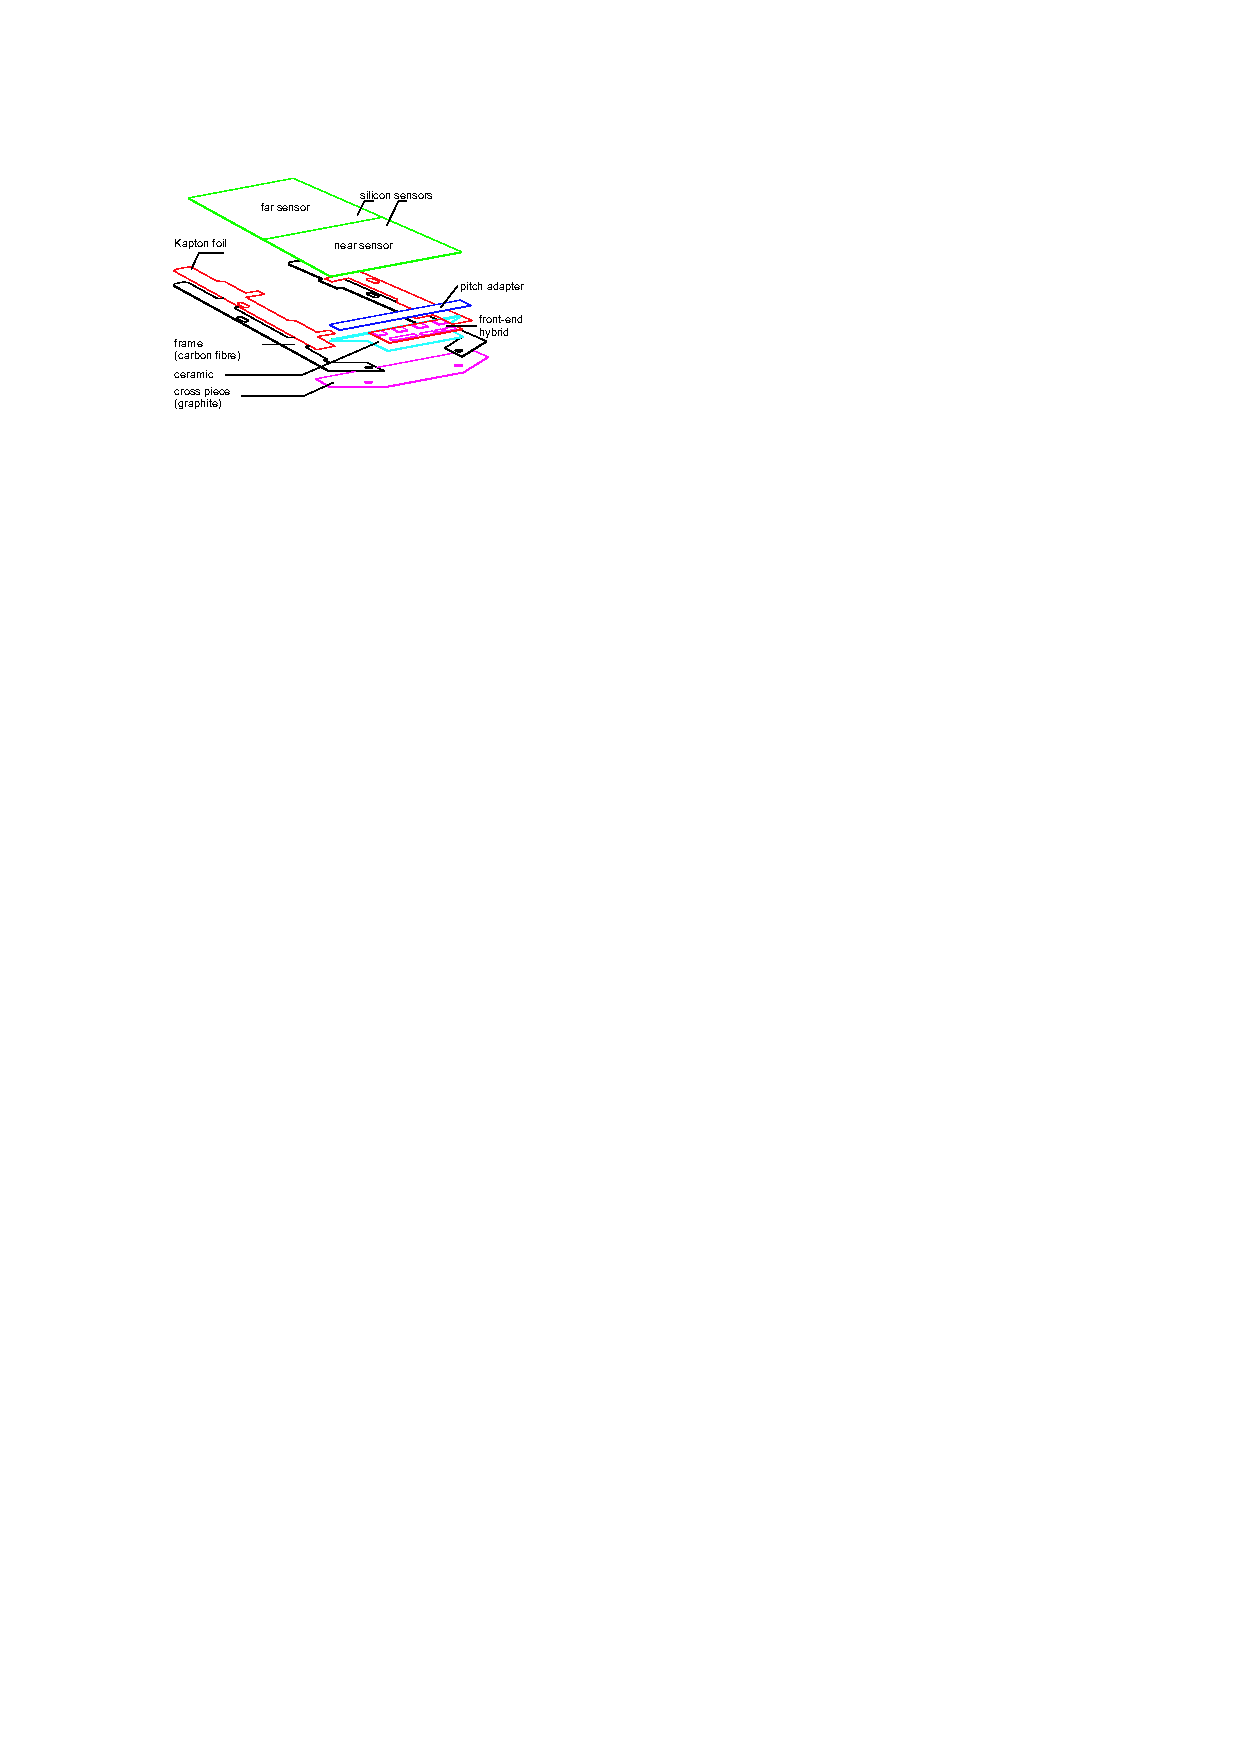
\includegraphics[scale=1.0]{tracker_module}
	\caption{Exploded view of a strip module with two sensors.  Reprinted from Fig. 3.22 of ref. \cite{CMS_detector_paper}.}
	\label{fig:tracker_module}
\end{figure}

\begin{figure}
	\centering
	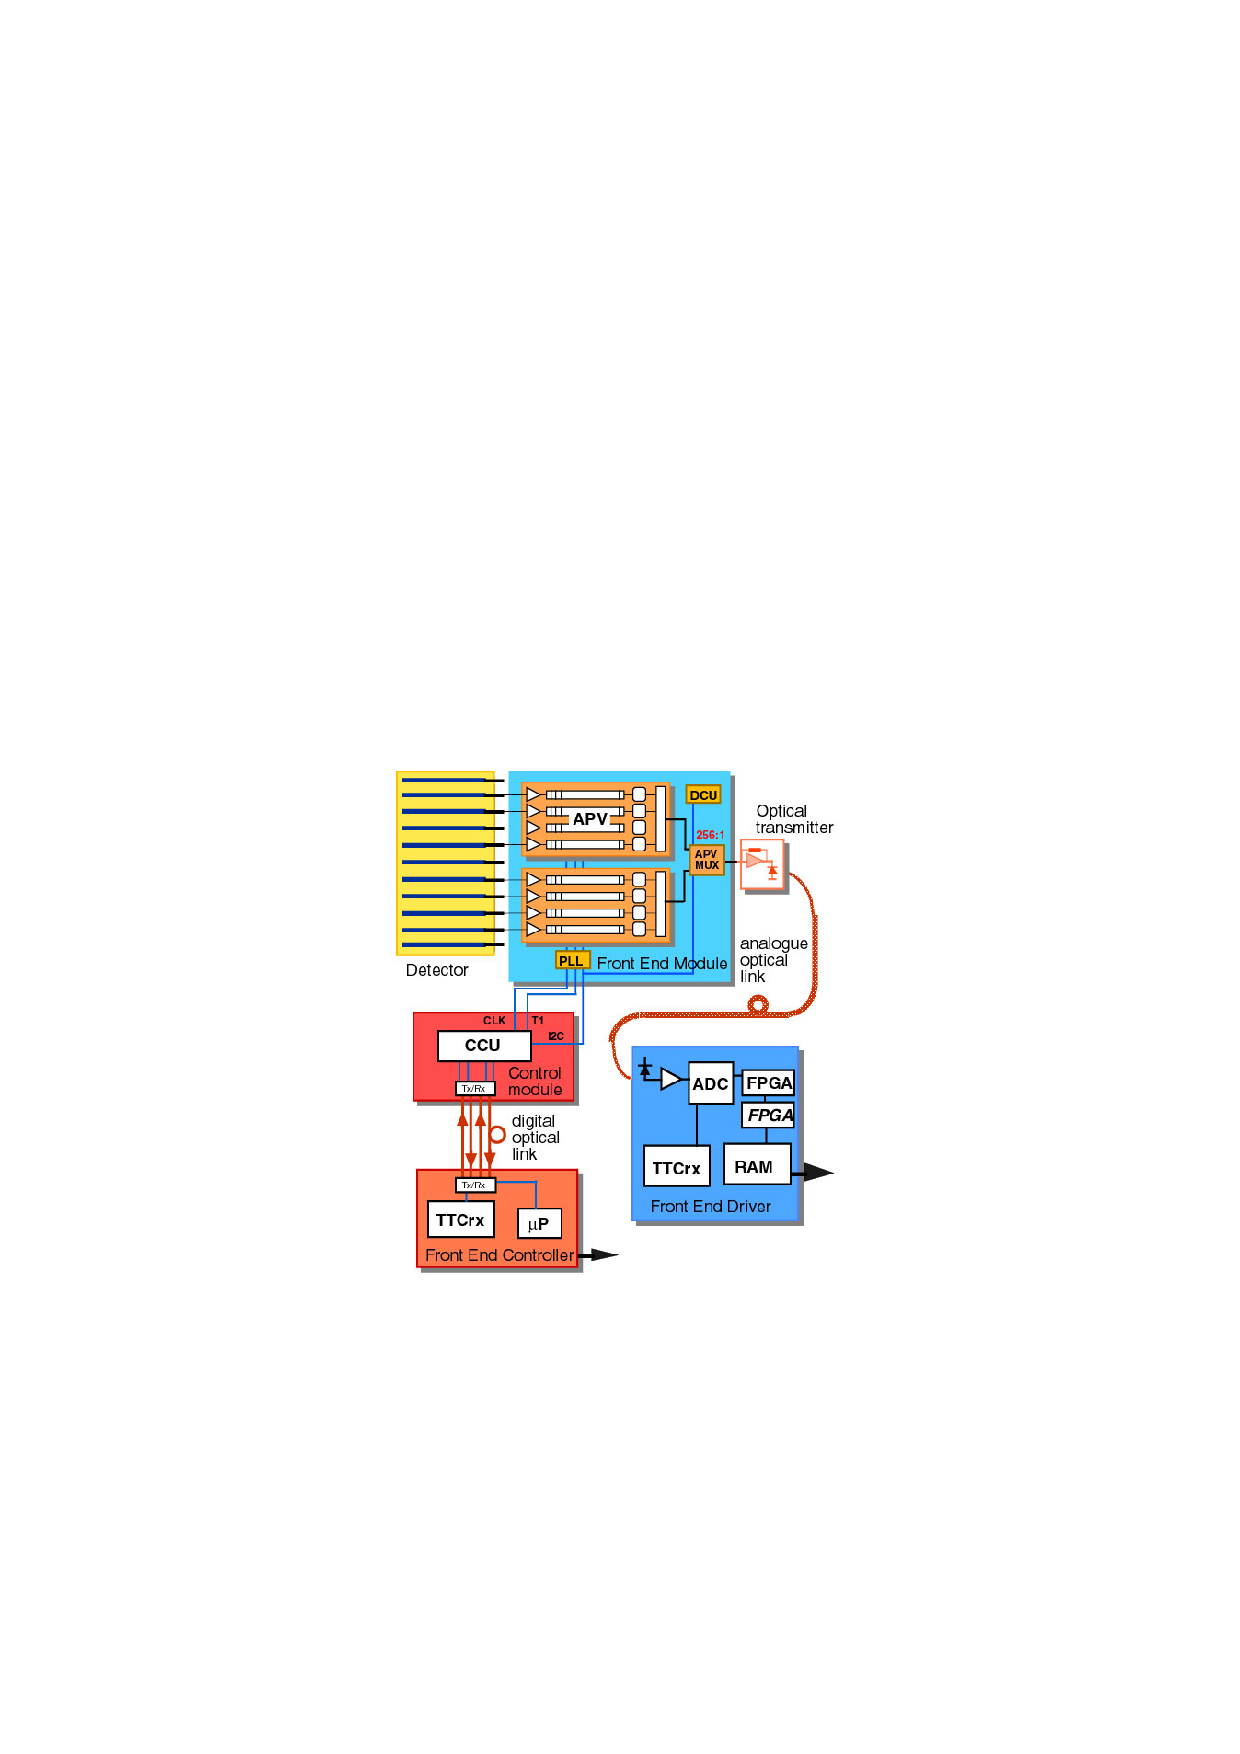
\includegraphics[scale=1.0]{tracker_readout}
	\caption{Block diagram of the strip readout architecture.  Reprinted from Fig. 3.20 of ref. \cite{CMS_detector_paper}.}
	\label{fig:tracker_readout}
\end{figure}

As an example of the strip capabilities, strip hit resolution and signal:noise measurements are shown in Figure~\ref{fig:tracker_results}.  The entire pixel + strip tracker has been used successfully in the reconstruction of primary and secondary vertices, electrons, muons, tau decays, and charm and bottom hadron decays.  In addition, the superior performance of the tracker over the hadronic calorimeter for low energy charged hadrons has been exploited in the the particle flow jet and \MET reconstruction technique (see Sec.~\ref{sec:Particle Flow}).  The CMS silicon strips, as well as the pixels, are well aligned and operating at close to design performance.  

\begin{figure}
	\centering
 	\subfloat[TIB signal:noise \cite{tracker_DPG_Twiki_TIB_SNR}.]{\label{fig:tracker_results_TIB_SNR}\includegraphics[scale=0.3]{tracker_results_TIB_SNR.gif}}
	\hspace{1cm}
	\subfloat[TIB and TOB hit resolution as a function of strip pitch \cite{tracker_DPG_Twiki_res}.]{\label{fig:tracker_results_res}\includegraphics[scale=0.2]{tracker_results_res.gif}}
	\caption{Strip detector performance highlights.}
	\label{fig:tracker_results}
\end{figure}

\subsection{Electromagnetic Calorimeter}
\label{sec:Electromagnetic Calorimeter}

The electromagnetic calorimeter (ECAL) is composed of 68,524 lead tungstate ($\mbox{PbWO}_{4}$) crystals, divided into one barrel (EB) layer and two endcap (EE) disks.  In EB, there are 1700 crystals per \textit{supermodule} (SM), arranged in a $20\times85$ grid in $\phi\times\eta$.  Two SMs are laid out end-to-end to form one row at fixed $\phi$, with a total of 18 rows needed to cover the entire $2\pi$ extent in $\phi$.  The SMs may be operated independently.  In EE, the independent unit is a wedge-shaped sector, with nine sectors covering each endcap side.  The 7,324 EE crystals are divided approximately evenly between the 18 EE sectors.  A two-layer preshower detector is placed in front of the EE disks, each layer consisting of a lead absorber followed by 1.9 mm pitch silicon strip detectors (the strips in the first layer are rotated $90^{\circ}$ with respect to the second layer).  The ECAL layout is shown in Figure~\ref{fig:ECAL_layout}.

\begin{figure}
	\centering
	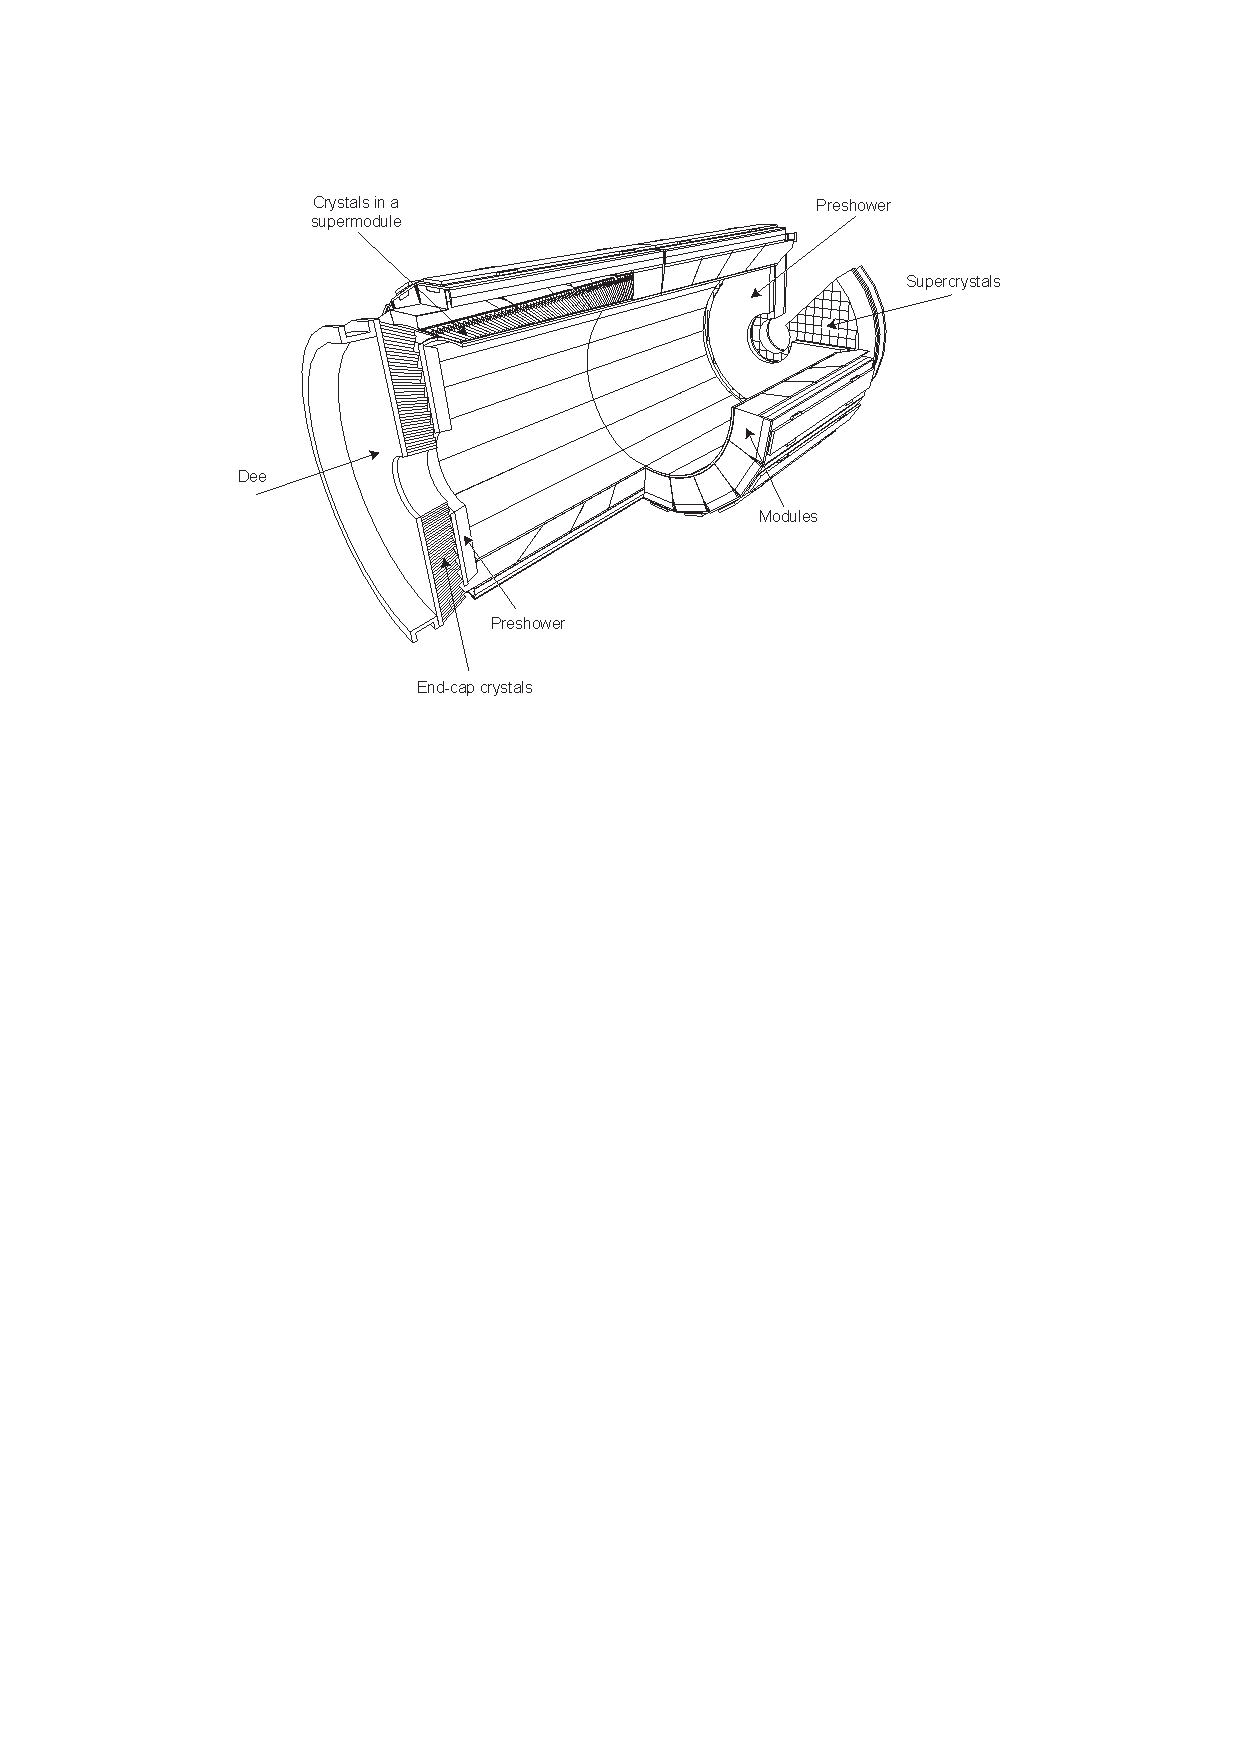
\includegraphics[scale=1.0]{ECAL_layout}
	\caption{Layout of the ECAL detector.  Reprinted from Fig. 4.5 of ref. \cite{CMS_detector_paper}.}
	\label{fig:ECAL_layout}
\end{figure}

The electromagnetic energy resolution can be parametrized as $(\sigma/E)^{2} = (S/\sqrt{E})^{2} + (N/E)^{2} + (C)^{2}$, where $S$ characterizes the size of photostatistical fluctuations, $N$ characterizes the contribution from electronics noise, and $C$ is a constant accounting for imperfect intercalibration between crystals, non-uniformity of crystal performance, and incomplete shower containment within one crystal.  The design goal of the ECAL is to achieve C = 0.5\%.  Therefore, fast, dense, and relatively radiation hard $\mbox{PbWO}_{4}$ was chosen as the crystal material.  When a photon or electron strikes the crystal, it initiates an electromagnetic (EM) shower.  Due to the density, short radiation length, and small Moli\`ere radius of $\mbox{PbWO}_{4}$, nearly the entirety of an EM shower can be contained in a single 23-cm long crystal with front face dimensions $2.2\mbox{ cm}\times2.2\mbox{ cm}$.  The crystals scintillate in the blue-green part of the spectrum, emitting $\sim80$\% of the scintillation light within 25 ns.  Light is transmitted along the length of the crystals and collected at the rear with avalanche photodiodes (semiconductor diodes) in EB or vacuum phototriodes (conventional photomultipliers) in EE.  Since the light output is low and varies with temperature, the crystals must be kept precisely at $18^{\circ}$C.  The EB and EE crystals, which are slightly tapered to match the lateral shower development, are shown in Figure~\ref{fig:ECAL_crystals}.

\begin{figure}
	\centering
	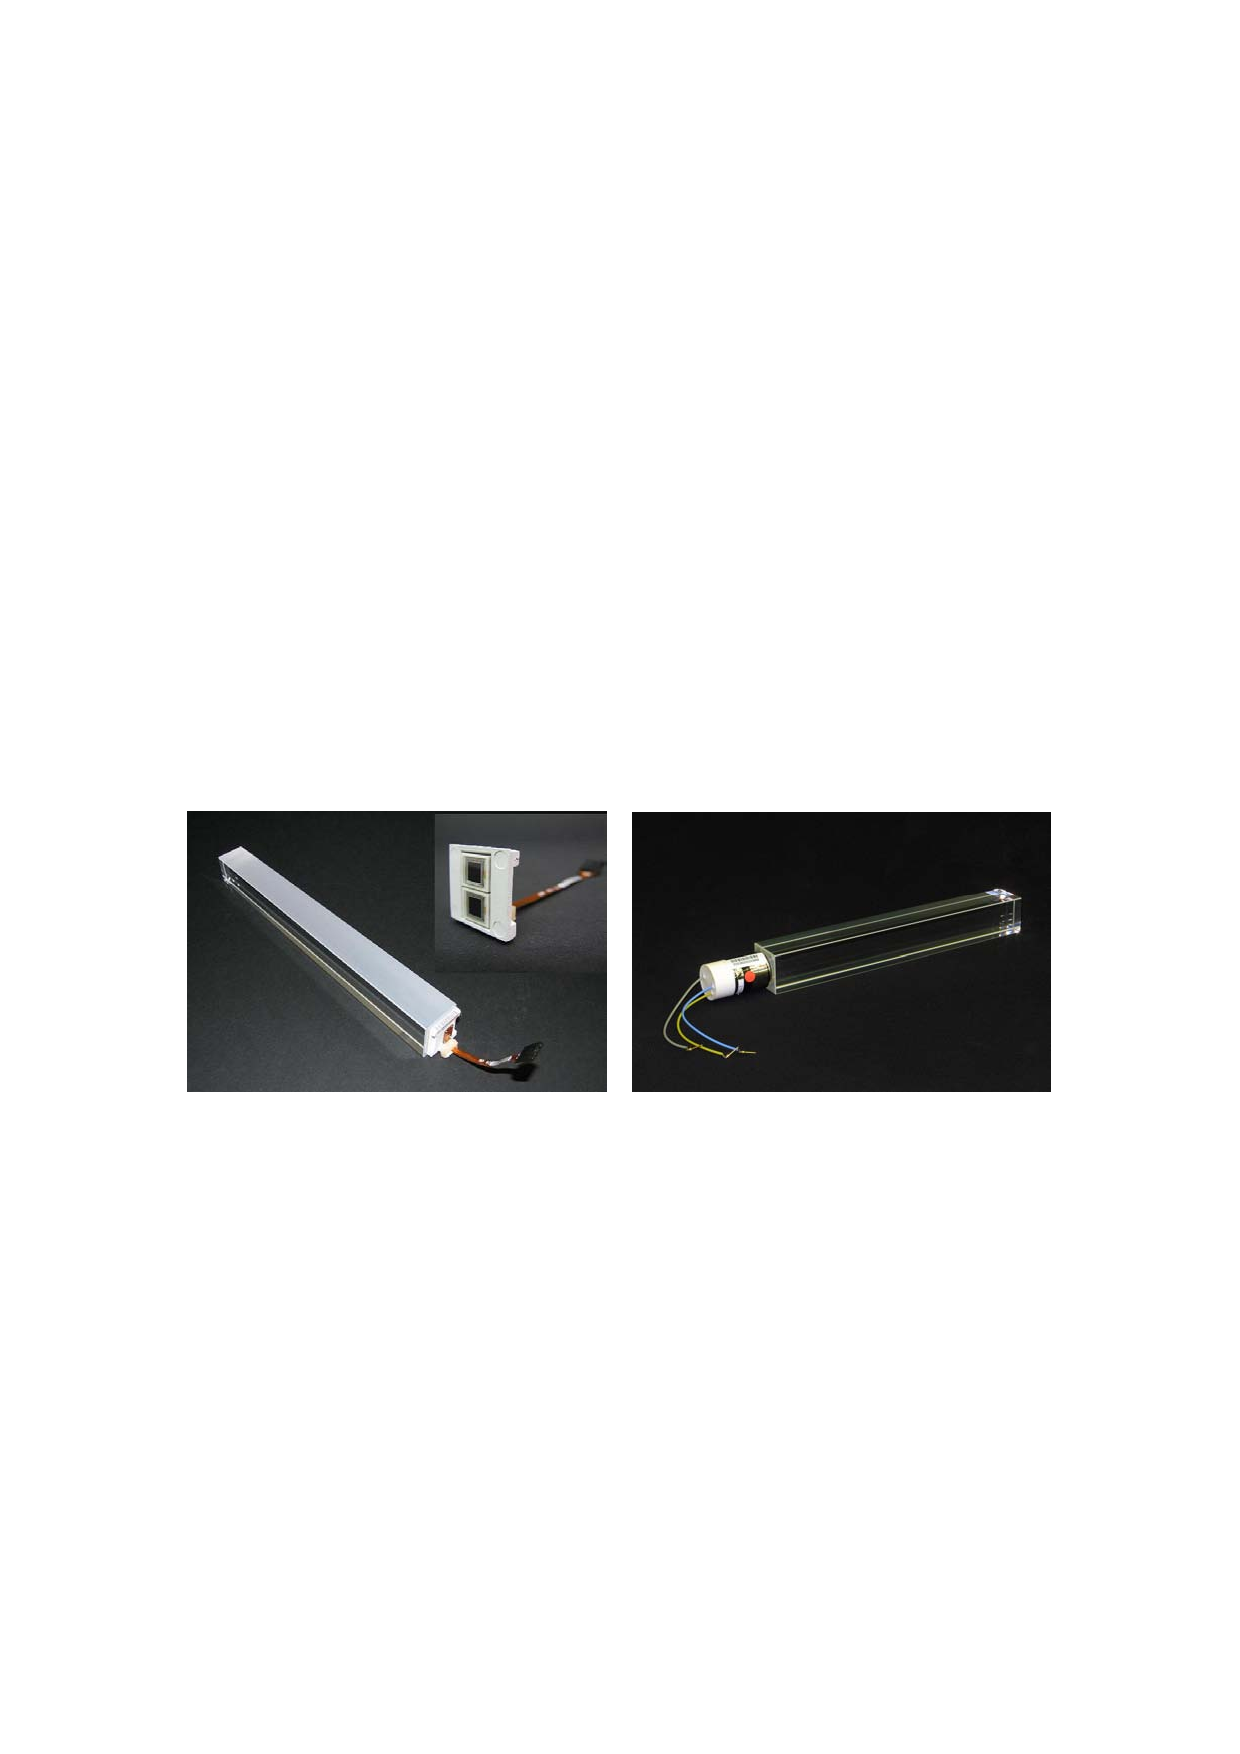
\includegraphics[scale=1.0]{ECAL_crystals}
	\caption{Left: EB crystal with attached APD.  Right: EE crystal with attached VPT.  Reprinted from Fig. 4.2 of ref. \cite{CMS_detector_paper}.}
	\label{fig:ECAL_crystals}
\end{figure}

For each trigger, 10 samples, each separated by 25 ns, are read out.  The 10-sample pulse is amplified and shaped by a multi-gain preamplifier (MGPA) residing on a very front end (VFE) card serving five crystals.  The MGPA can switch between gains 1, 6, and 12 to avoid saturation of the electronics, and affords a dynamic range up to 3 TeV.  The samples are digitized on the VFE card, then sent to the front end (FE) card serving five VFEs.  Digitized samples are buffered in the FE card until receipt of a trigger, when they are sent over an optical link to the data concentrator card (DCC) that interfaces to the global DAQ.  The DCC interfaces to the \textit{selective readout} processor, which decides whether a crystal should be read out with or without zero suppression based on its proximity to a high-energy hit.  The clock is transmitted to the FE cards from the Clock and Control System (CCS) boards.  A flow chart of the crystal readout is given in Figure~\ref{fig:ECAL_readout}.

\begin{figure}
	\centering
	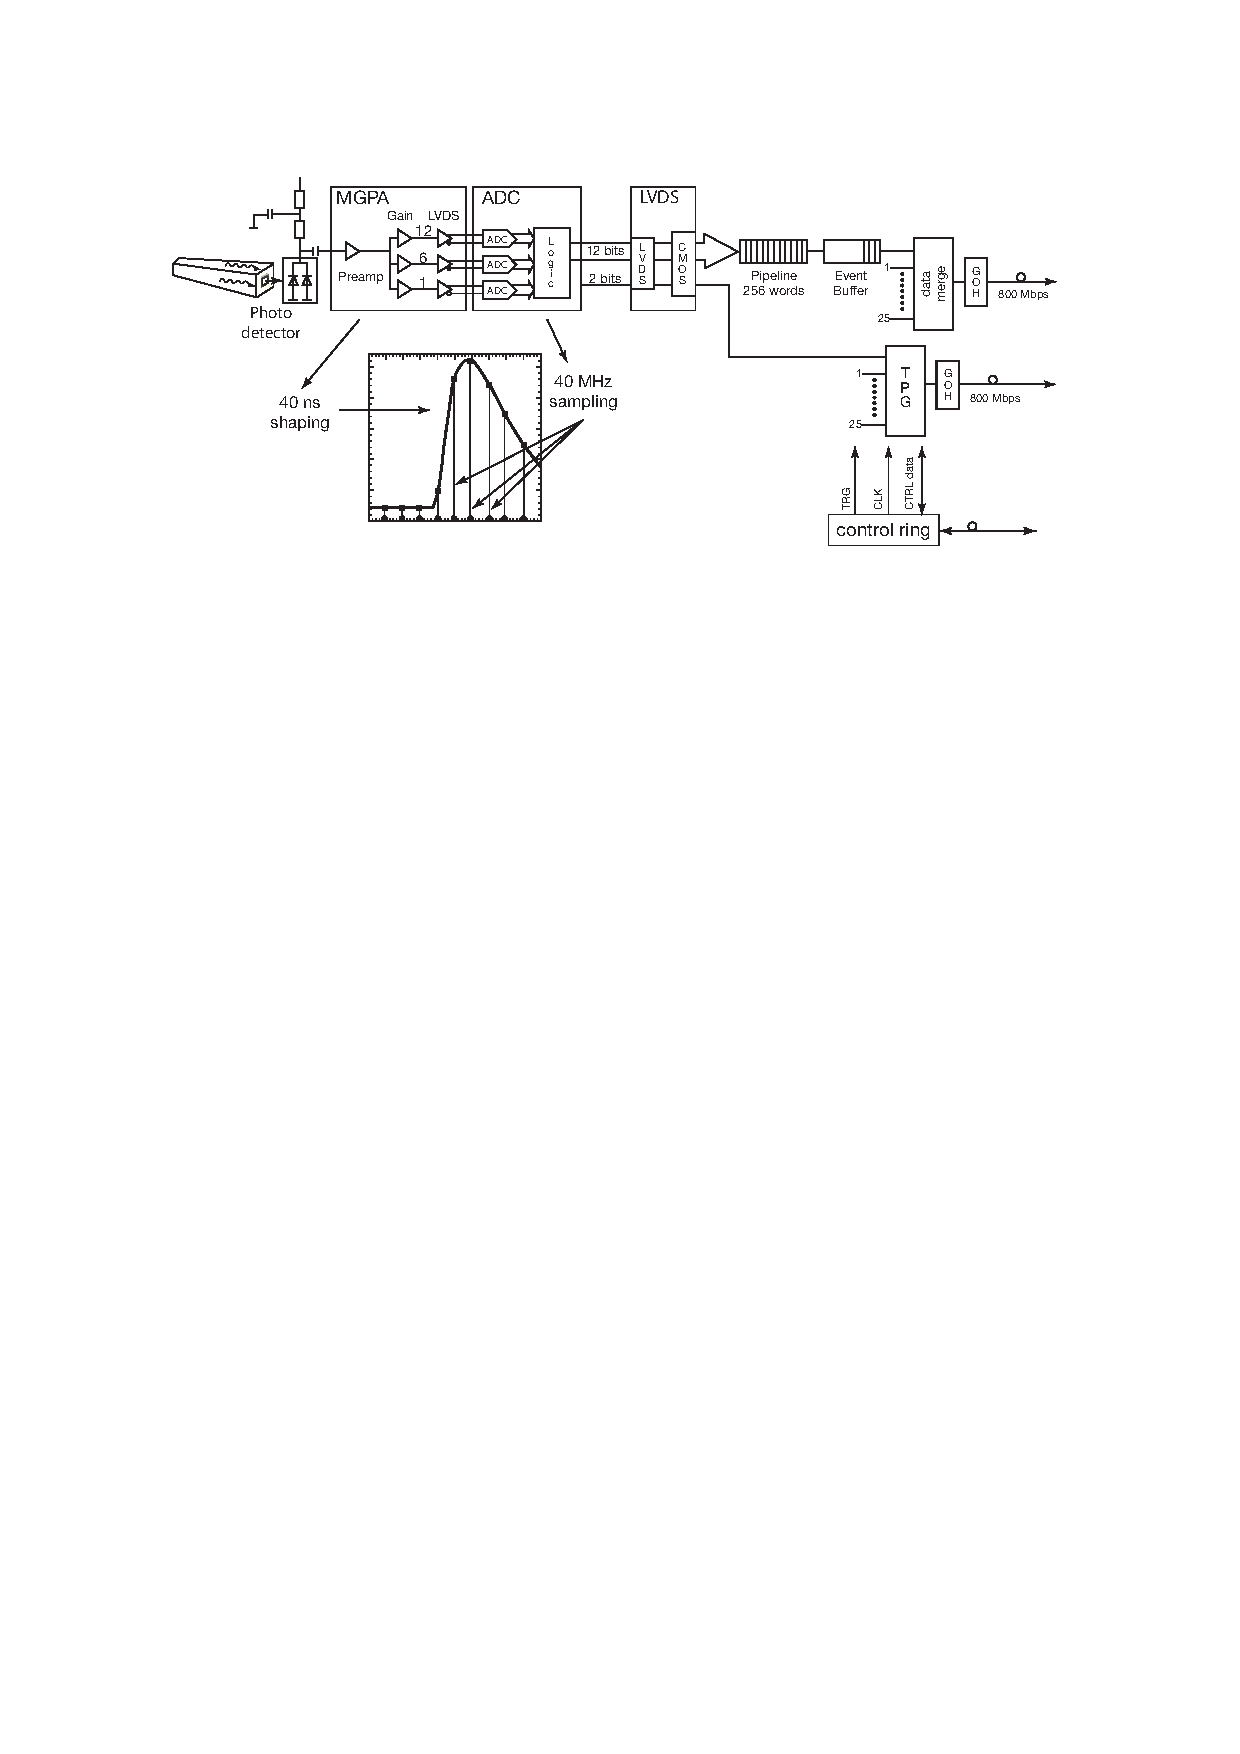
\includegraphics[scale=1.0]{ECAL_readout}
	\caption{Flow chart of the crystal readout, showing the 10-sample pulse shape.  Reprinted from Fig. 4.9 of ref. \cite{CMS_detector_paper}.}
	\label{fig:ECAL_readout}
\end{figure}

At each bunch crossing, the trigger concentrator cards (TCC) of the ECAL compute \textit{trigger primitives} from $5\times5$ non-overlapping transverse energy sums (in the endcaps the geometry is not always $5\times5$).  This information, along with a special bit in EB only characterizing the transverse shower profile that is used for rejection of anomalous APD hits (see Sec.~\ref{sec:Calibrated EB/EE Hits}), is transmitted from the TCCs to the synchronization and link boards (SLBs), and then on to the global trigger system.  The trigger decision is communicated to the DCCs, which request the buffered data from the front ends if the decision is affirmative.

Despite the radiation hardness of lead tungstate relative to other types of crystals, it still suffers from transparency loss due to radiation-induced lattice damage, as shown in Figure~\ref{fig:ECAL_rad_damage}.  In addition, any unforeseen change in the gains of the MGPAs and VPTs, or in the pedestal levels, will degrade the energy resolution.  For this reason, a continuously running calibration system is installed with the ECAL.  The system makes use of the LHC abort gaps to read out the pedestal levels, test pulses fired into the MGPAs, and laser (EB and EE) or LED (EE only) pulses fired into the crystals at regular intervals.  Laser and LED events are used to compute corrections to the crystal gains for transparency loss, while the other types of calibration events serve to monitor changes in the electronics performance due to magnetic field or high voltage cycling.  The mean time between transparency measurements is $\sim40$ minutes.  Figure~\ref{fig:ECAL_laser_system} shows the architecture of the laser monitoring system.

\begin{figure}
	\centering
	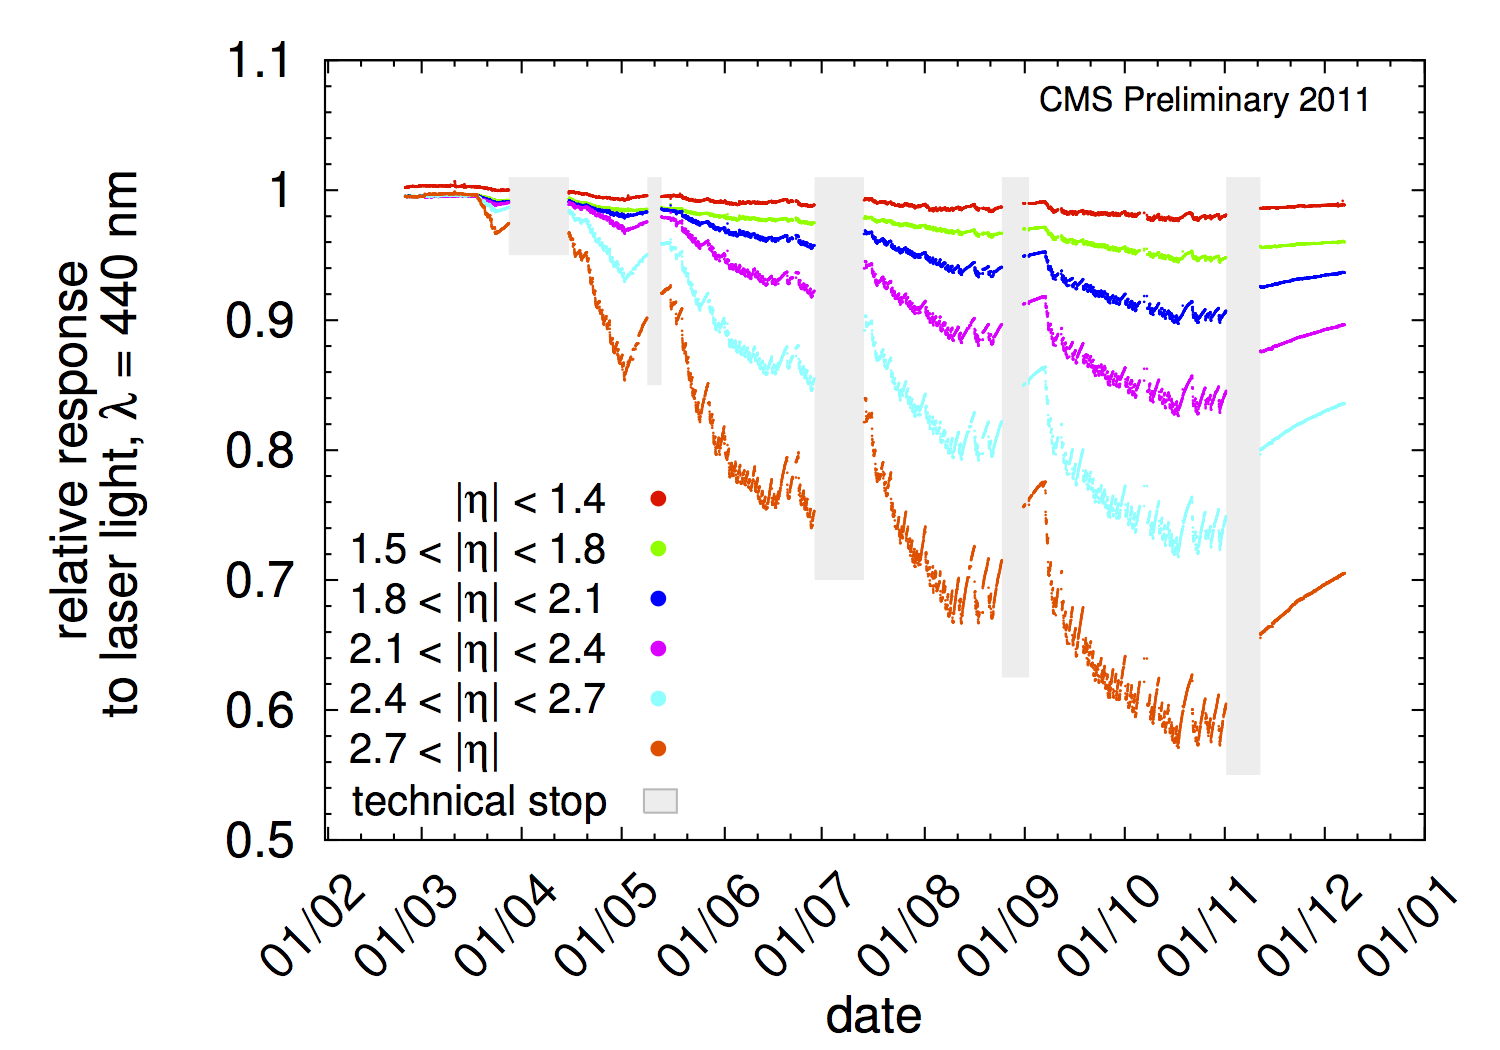
\includegraphics[scale=1.0]{ECAL_rad_damage}
	\caption{Relative response of the crystals to blue laser pulses from February 1, 2011 to January 1, 2012 \cite{ECAL_DPG_Twiki_rad_damage}.  Technical stops, during which the LHC is turned off for maintenance and development, are shown in gray.  These periods of inactivity correspond to growth in the crystal response, as radiation damage recovery occurs.}
	\label{fig:ECAL_rad_damage}
\end{figure}

\begin{figure}
	\centering
	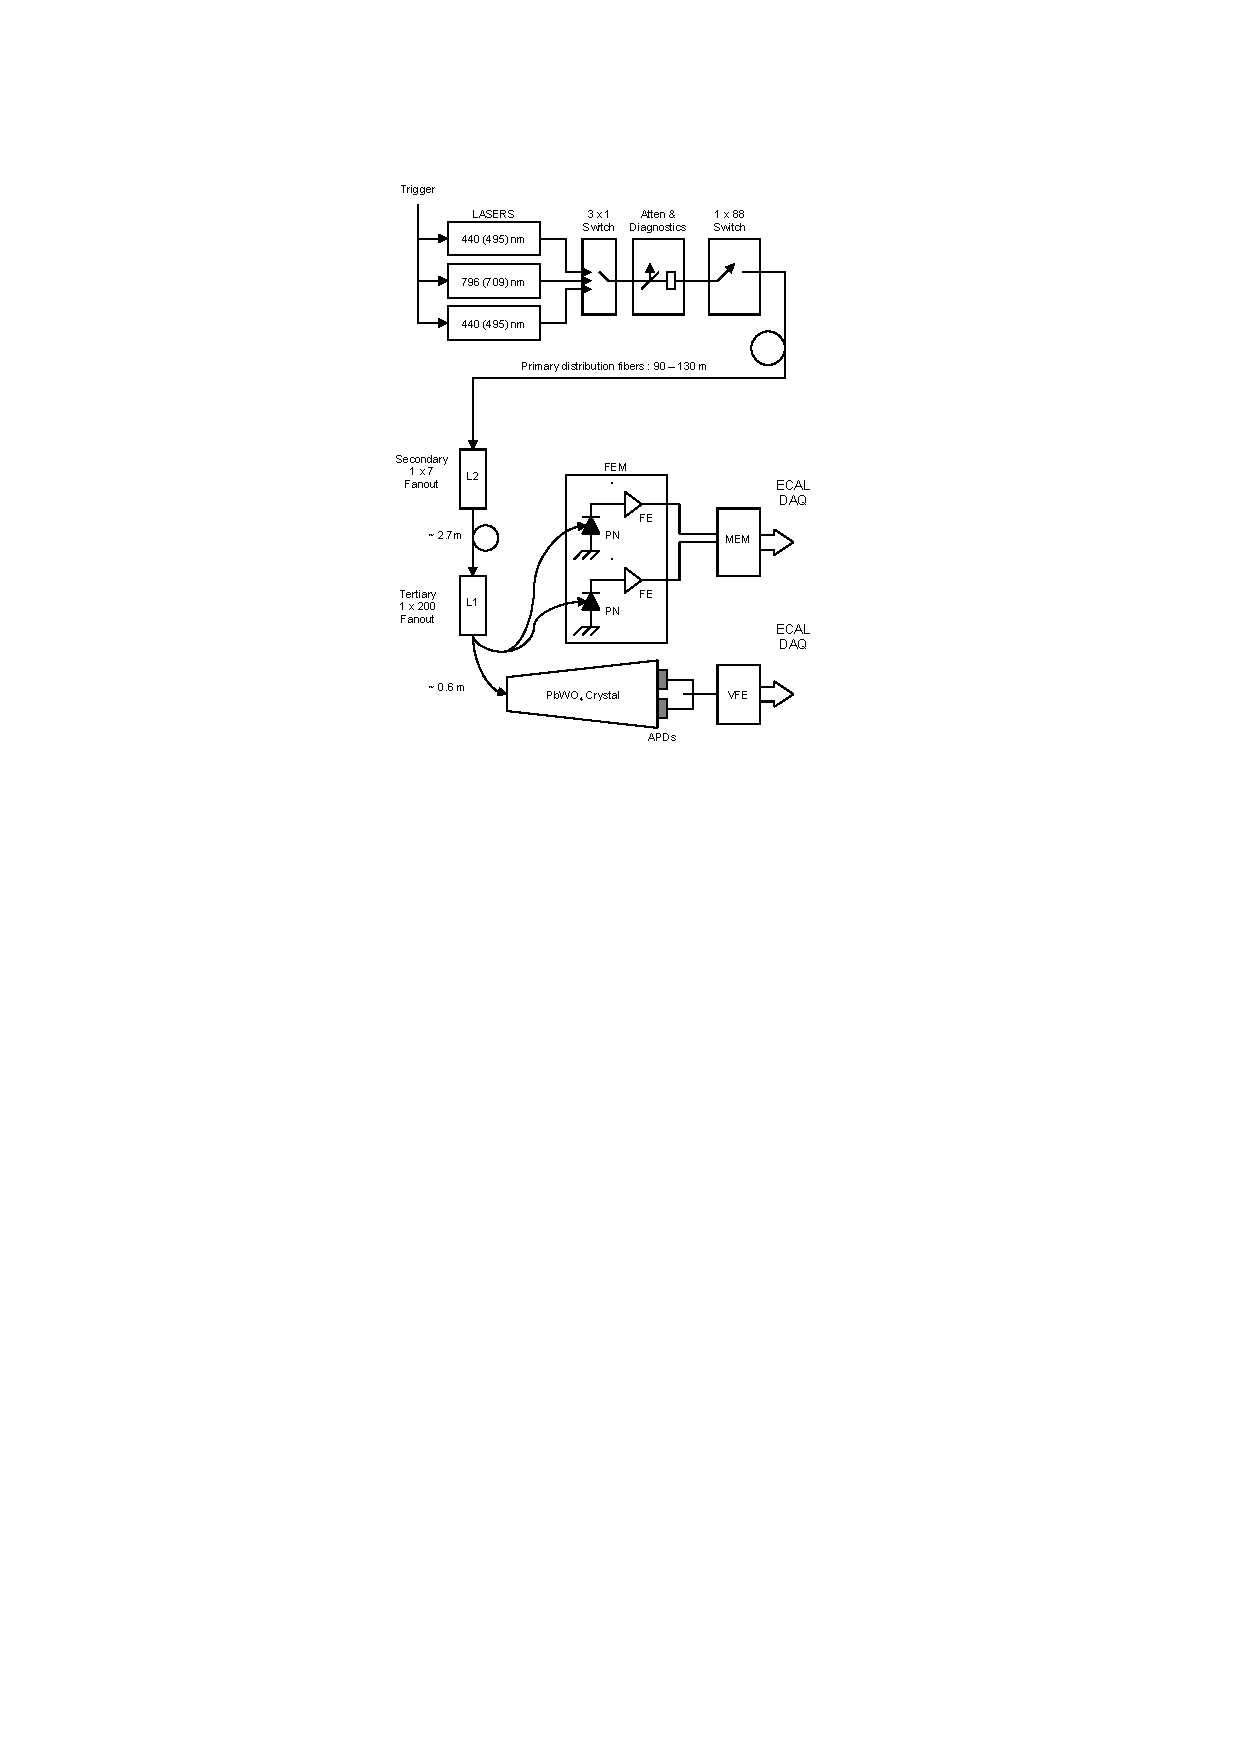
\includegraphics[scale=1.0]{ECAL_laser_system}
	\caption{Architecture of the laser monitoring system.  Reprinted from Fig. 4.16 of ref. \cite{CMS_detector_paper}.}
	\label{fig:ECAL_laser_system}
\end{figure}

The current ECAL energy resolution is somewhat worse than the design goal of 0.5\%.  An incomplete understanding of the transparency loss is the main limiting factor in improving the resolution.  However, as more radiation damage data accumulate, more refined models of transparency loss can be built, leading to better resolution.  Energy resolution vs. $|\eta|$ can be seen in Figure~\ref{fig:ECAL_res_vs_eta}.

\begin{figure}
	\centering
 	\subfloat[EB \cite{ECAL_DPG_Twiki_res_vs_eta_EB}.]{\label{fig:ECAL_res_vs_eta_EB}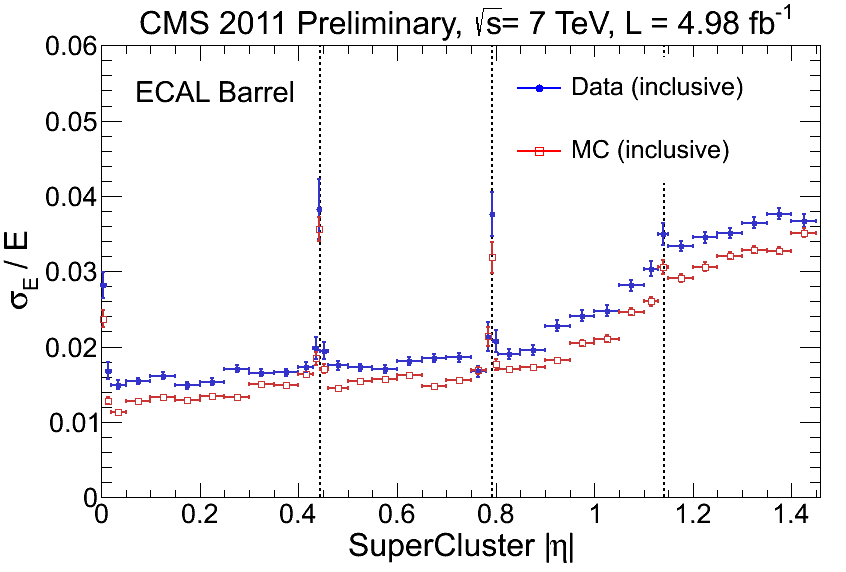
\includegraphics[scale=0.2]{ECAL_res_vs_eta_EB}}
	\hspace{1cm}
	\subfloat[EE \cite{ECAL_DPG_Twiki_res_vs_eta_EE}.]{\label{fig:ECAL_res_vs_eta_EE}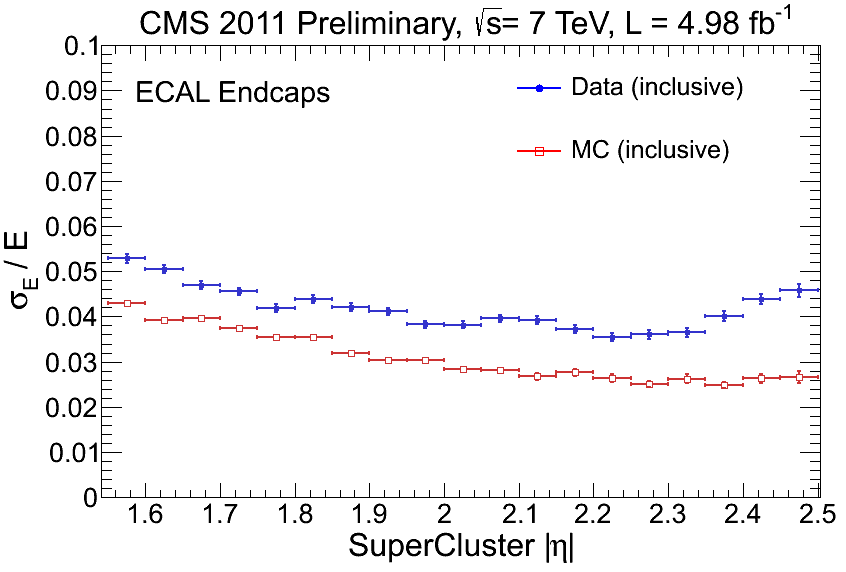
\includegraphics[scale=0.2]{ECAL_res_vs_eta_EE}}
	\caption{Energy resolution vs. $|\eta|$ for $Z$ decay electrons for data (blue) and MC (red).  The dotted lines show the locations of module gaps (three per SM).}
	\label{fig:ECAL_res_vs_eta}
\end{figure}

The 10-sample readout coupled with the fast scintillation time of lead tungstate allows for a very precise reconstruction of the time of ECAL hits.  ECAL timing is used for searches for long-lived particles that decay to photons or jets, such as long-lived neutralinos in GMSB \cite{long-lived_GMSB_paper}.  Figure~\ref{fig:ECAL_timing_res} shows the timing resolution in EE.

\begin{figure}
	\centering
	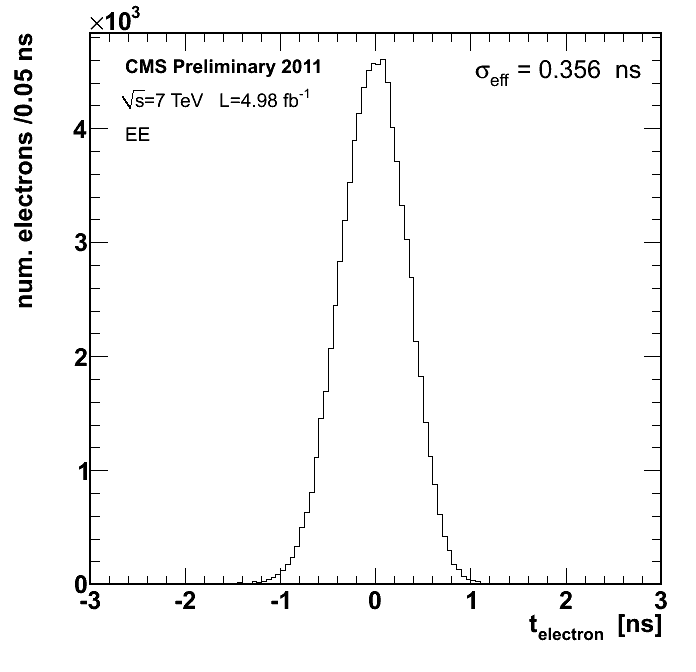
\includegraphics[scale=0.3]{ECAL_timing_res}
	\caption{Distribution of reconstructed times of $Z$ decay electrons in EE \cite{ECAL_DPG_Twiki_timing_res}.}
	\label{fig:ECAL_timing_res}
\end{figure}

\subsection{Hadronic Calorimeter}

%layout of the detector (names of the sub-parts, technologies used)
%explanation of how the technology works and short motivation for choosing it
%short explanation of the readout (discuss crystal radiation damage monitoring)
%if the detector triggers, explanation of the trigger primitive generation
%performance benchmarks

\subsection{Muon System}
%spend very little time on this

\section{Triggering, Data Acquisition, and Data Transfer}
\label{sec:Triggering, Data Acquisition, and Data Transfer}

\subsection{Level 1 and High Level Trigger Systems}
\label{sec:Level 1 and High Level Trigger Systems}
%talk about trigger primitives for the ECAL especially (there is a reference to this section from the HLT section in ch. 6 when we talk about L1 seeds), SR, etc.
\subsection{Data Acquisition System}
\subsection{Data Processing and Transfer to Computing Centers}
\label{sec:Data Processing and Transfer to Computing Centers}
%define lumi section

Lorum ipsum fuck Republicans.

\end{document}